\newcommand{\shapefigurepartbase}[4]{
  \begin{subfigure}{0.2\textwidth}
    \includegraphics[width=\linewidth]{assets/images/shapes/#2/#1#3}
    \caption{\makefirstuc{#2 #4}.}
    \label{fig:#2_#1#3}
  \end{subfigure}
}

\newcommand{\shapefigurepartbasealt}[4]{
  \begin{subfigure}{0.4\textwidth}
    \includegraphics[width=\linewidth]{assets/images/shapes/#2/#1#3}
    \caption{\makefirstuc{#2 #4}.}
    \label{fig:#2_#1#3}
  \end{subfigure}
}

\newcommand{\shapefigurepart}[2]{
  \shapefigurepartbase{#1}{#2}{}{model}
}
\newcommand{\shapefigurepartalt}[2]{
  \shapefigurepartbasealt{#1}{#2}{}{model}
}

\newcommand{\shapefigurepartw}[2]{
  \shapefigurepartbase{#1}{#2}{_w}{wireframe}
}

\newcommand{\shapefigurepartwalt}[2]{
  \shapefigurepartbasealt{#1}{#2}{_w}{wireframe}
}

\newcommand{\shapefigure}[2]{
\begin{figure}
  \begin{center}
    \shapefigurepart{#1}{old}
    \shapefigurepartw{#1}{old}
    \shapefigurepart{#1}{new}
    \shapefigurepartw{#1}{new}
  \end{center}
  \caption{\makefirstuc{#2 molecule mesh implementation.}}
  \label{fig:#1_shape}
\end{figure}
}

\newcommand{\oldshapefigure}[1]{
\begin{figure}
  \begin{center}
    \shapefigurepart{#1}{old}
    \shapefigurepartw{#1}{old}
  \end{center}
  \caption{\makefirstuc{#1}.}
  \label{fig:#1_shape}
\end{figure}
}

\newcommand{\newshapefigure}[2]{
\begin{figure}
  \begin{center}
    \shapefigurepartalt{#1}{new}
    \shapefigurepartwalt{#1}{new}
  \end{center}
  \caption{\makefirstuc{#2}.}
  \label{fig:#1_shape}
\end{figure}
}

\section{Shapes}
\label{shapes_section}
\subsection{WebMGA 2.0 Implementation}
WebMGA 2.0 implements the following molecule shapes:
\begin{itemize}
  \item Sphere (\cref{fig:sphere_shape})
  \item Ellipsoid (\cref{fig:ellipsoid_shape})
  \item Spherocylinder (\cref{fig:spherocylinder_shape})
  \item Spheroplatelet (\cref{fig:spheroplatelet_shape})
  \item Cut Sphere (\cref{fig:doublecutsphere_shape}, implemented as a double cut sphere)
  \item Cylinder (\cref{fig:cylinder_shape})
  \item Torus (\cref{fig:torus_shape})
\end{itemize}
Notably missing but useful are the single cut sphere, the spherical cap, and the lens. The cylinder and torus shapes are present since the three.js library provides easily callable predefined meshes, however serve little practical purpose since no realistic molecular configuration would model using these.
\oldshapefigure{cylinder}
\oldshapefigure{torus}

\subsection{WebMGA 2.0 Bugs}
Some bugs in the existing shape geometries are shown in \cref{fig:bad_spherocylinder_old,fig:uneven_mesh_old,fig:no_height_bug_old}.
\begin{figure}
  \begin{center}
    \begin{subfigure}{0.24\textwidth}
    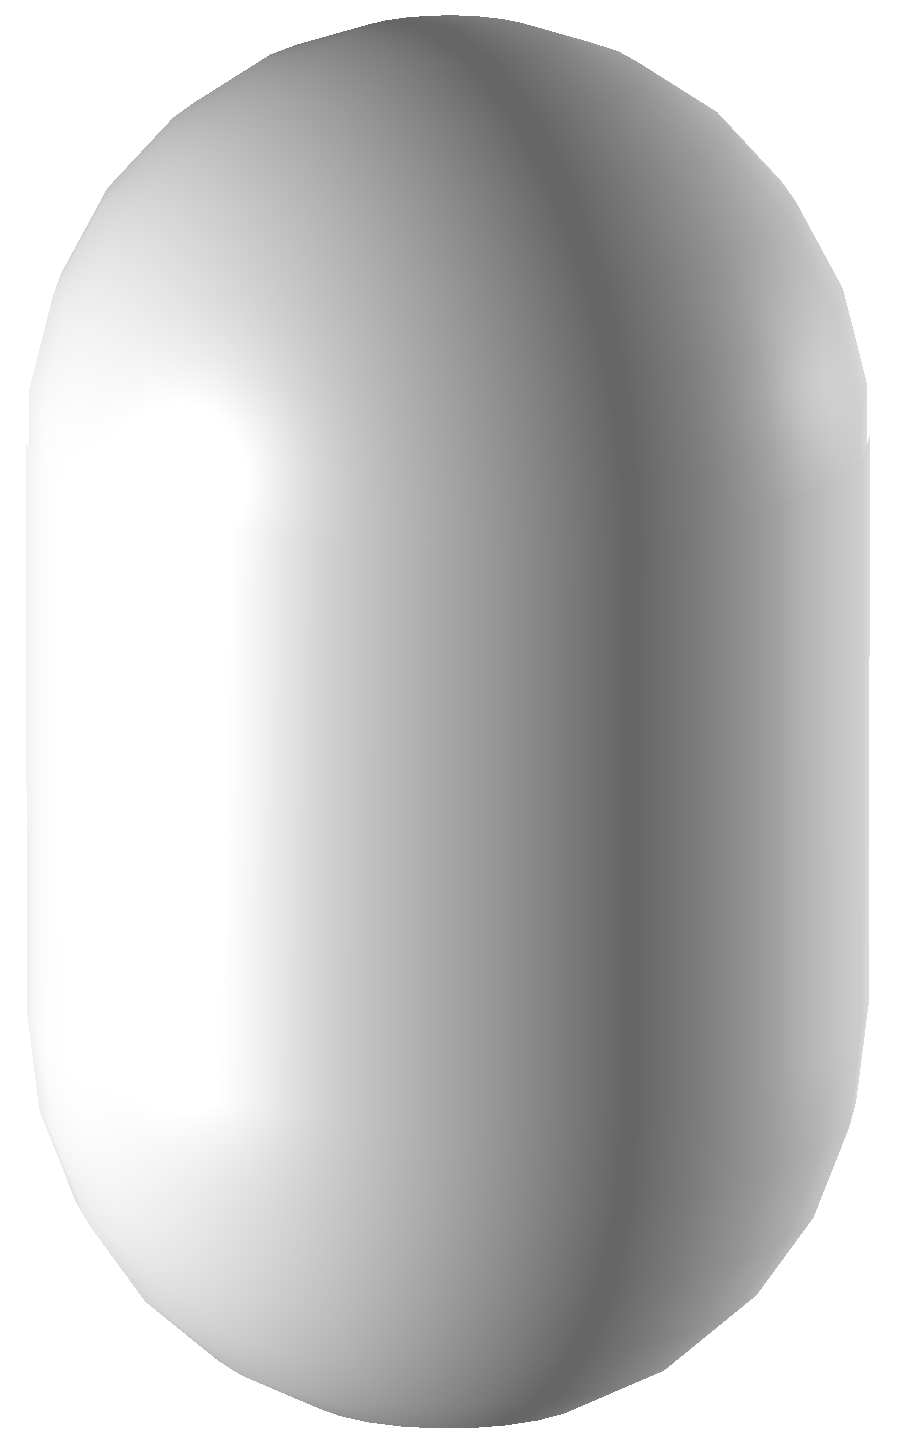
\includegraphics[width=\linewidth]{assets/images/shapes/bugold/bad_mesh_high}
    \caption{\makefirstuc{High detail shape.}}
    \end{subfigure}
      \begin{subfigure}{0.24\textwidth}
    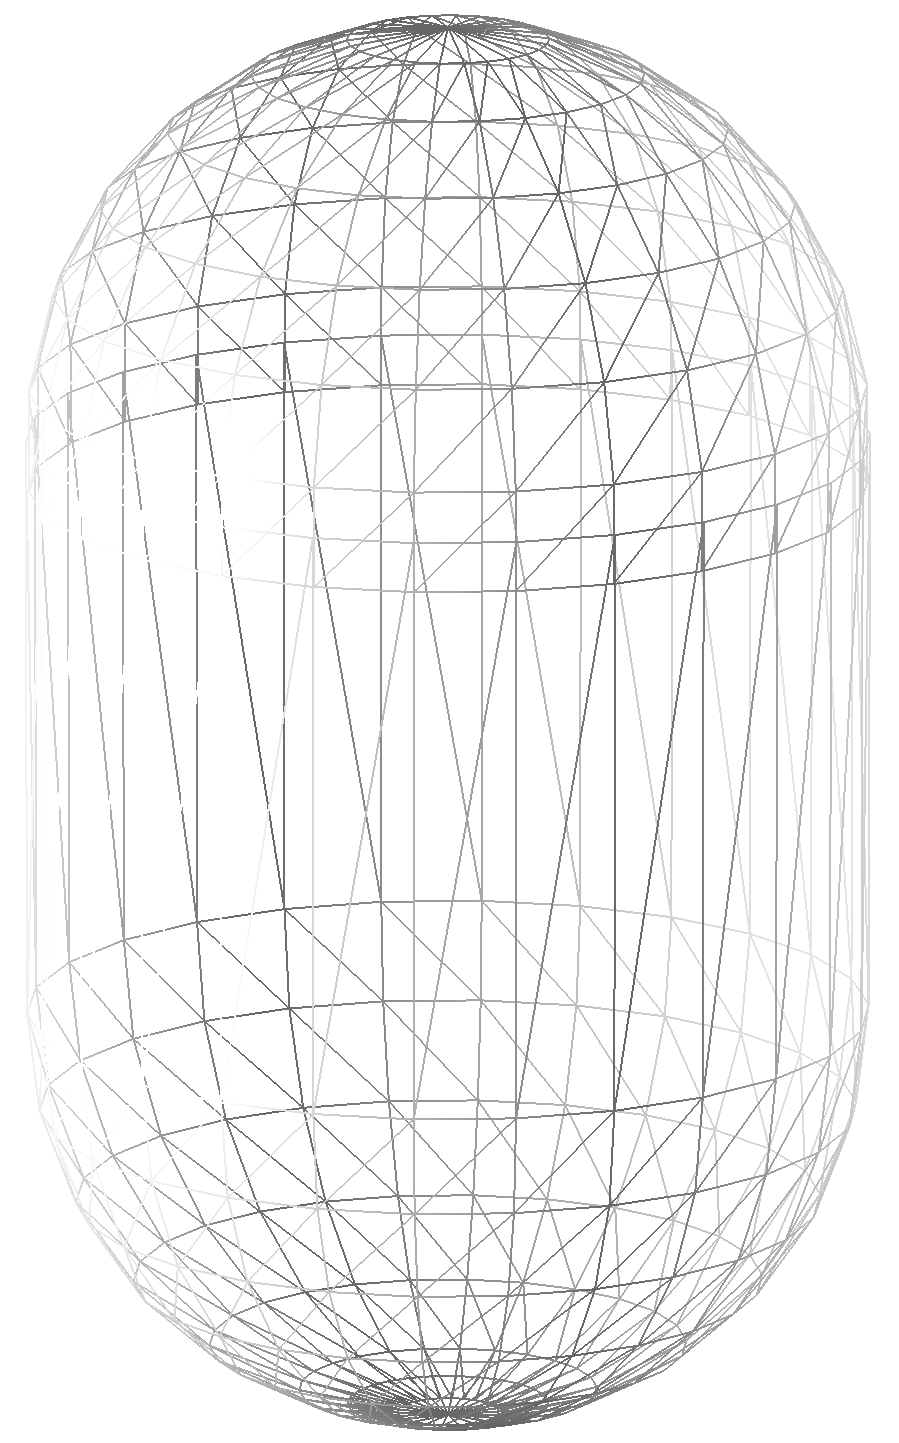
\includegraphics[width=\linewidth]{assets/images/shapes/bugold/bad_mesh_high_w}
    \caption{\makefirstuc{High detail mesh.}}
    \end{subfigure}
    \begin{subfigure}{0.24\textwidth}
    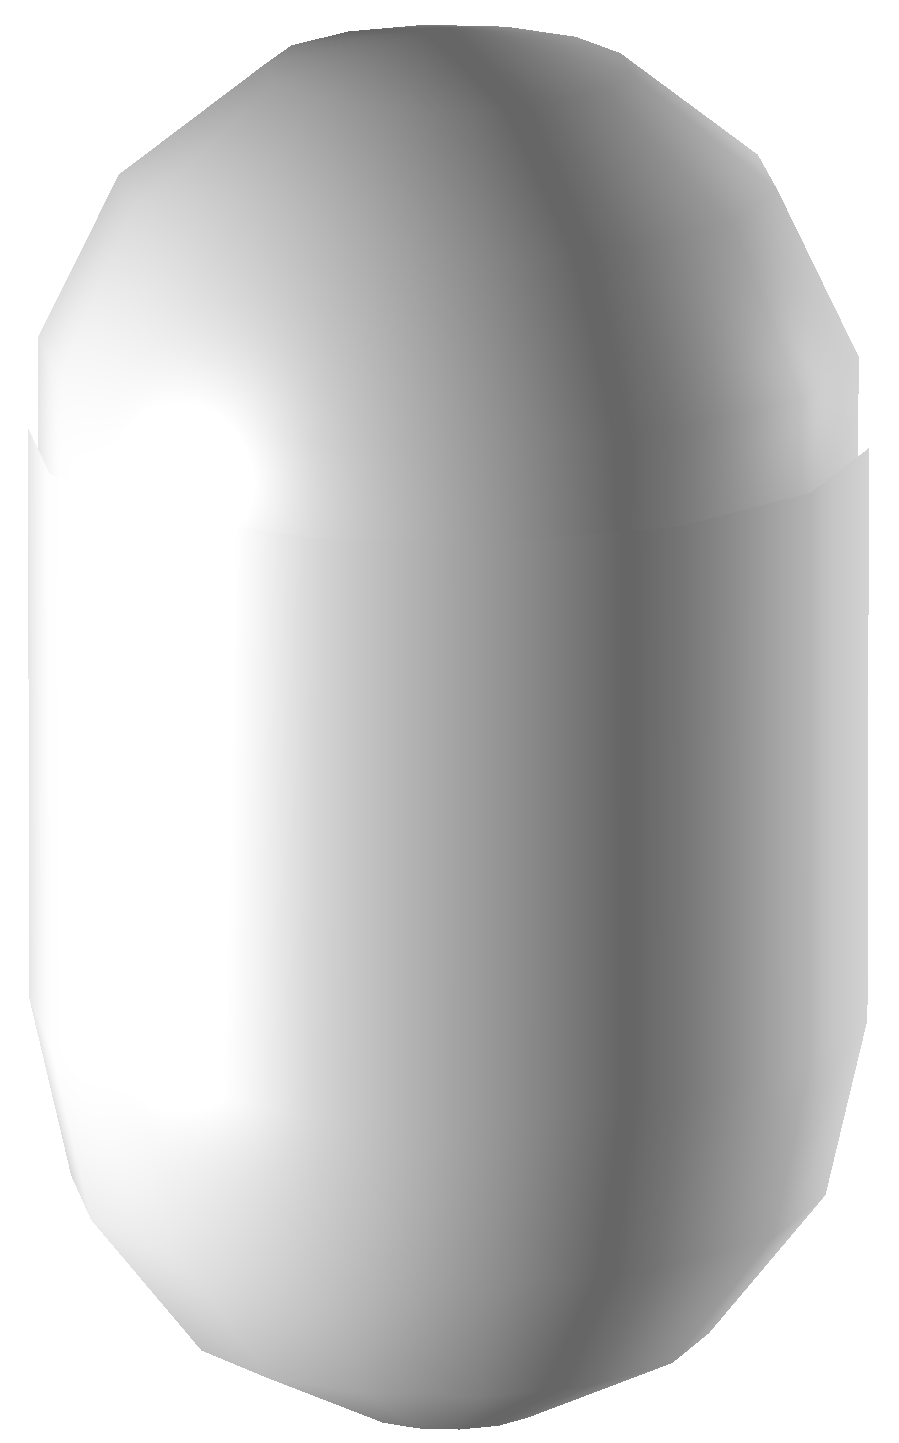
\includegraphics[width=\linewidth]{assets/images/shapes/bugold/bad_mesh_med}
    \caption{\makefirstuc{Mid detail shape.}}
    \end{subfigure}
    \begin{subfigure}{0.24\textwidth}
    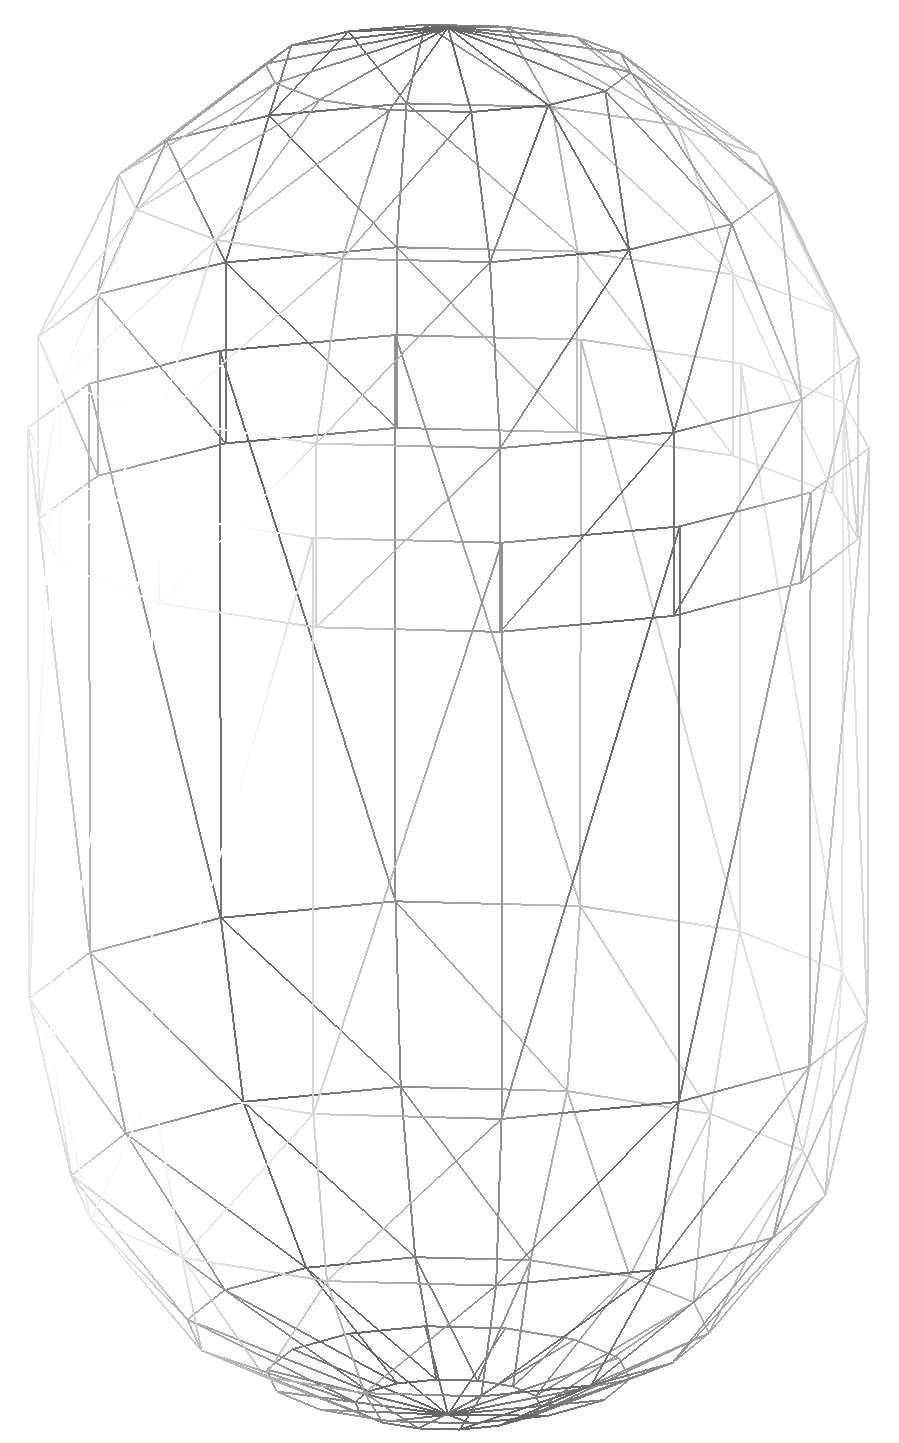
\includegraphics[width=\linewidth]{assets/images/shapes/bugold/bad_mesh_med_w}
    \caption{\makefirstuc{Mid detail mesh.}}
    \end{subfigure}
    \begin{subfigure}{0.24\textwidth}
    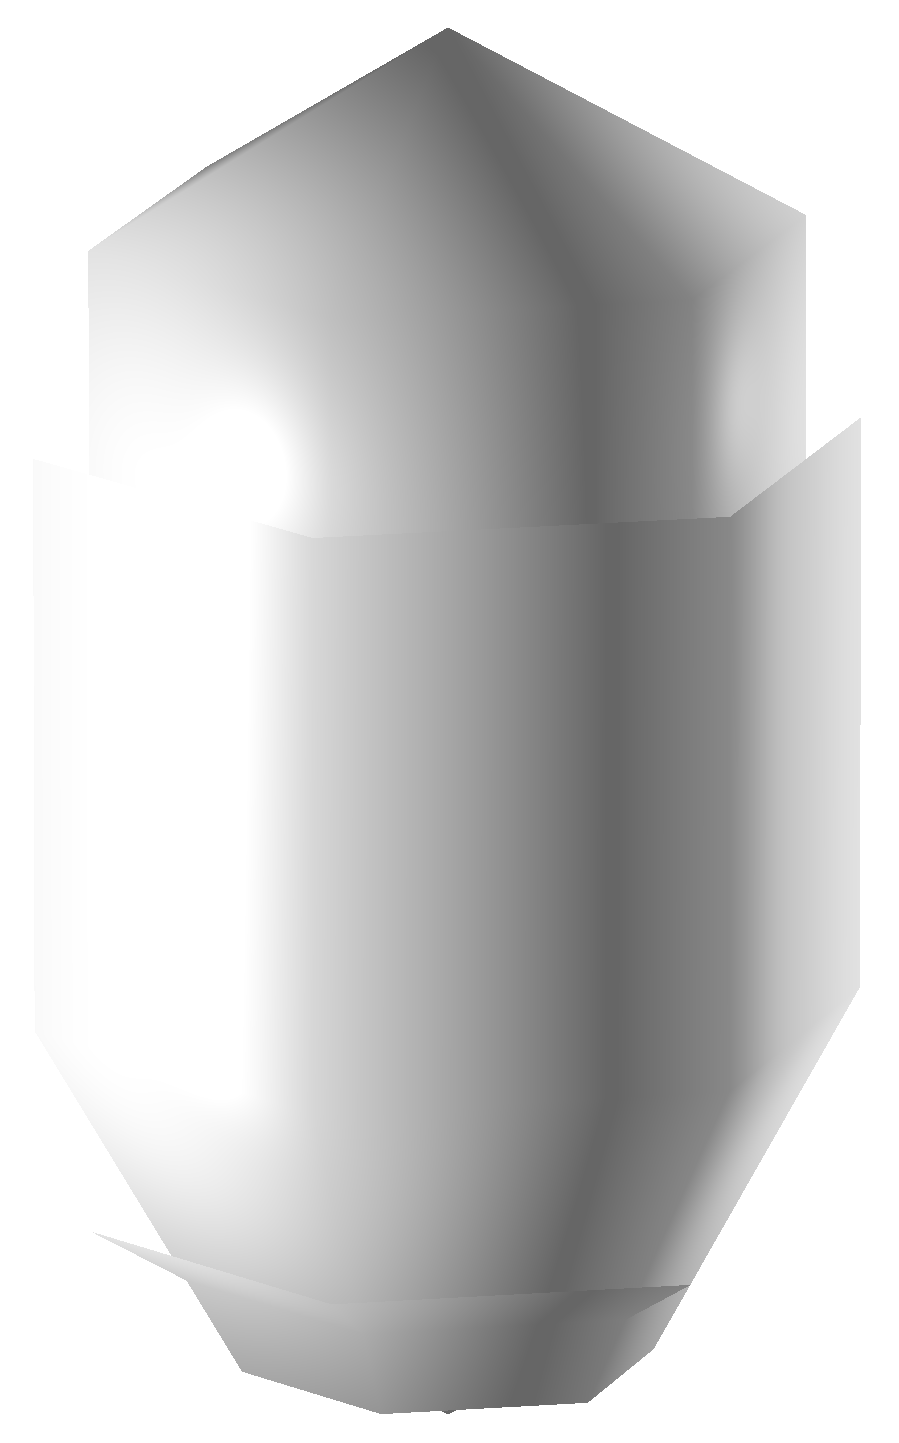
\includegraphics[width=\linewidth]{assets/images/shapes/bugold/bad_mesh_low}
    \caption{\makefirstuc{Low detail shape.}}
    \end{subfigure}
    \begin{subfigure}{0.24\textwidth}
    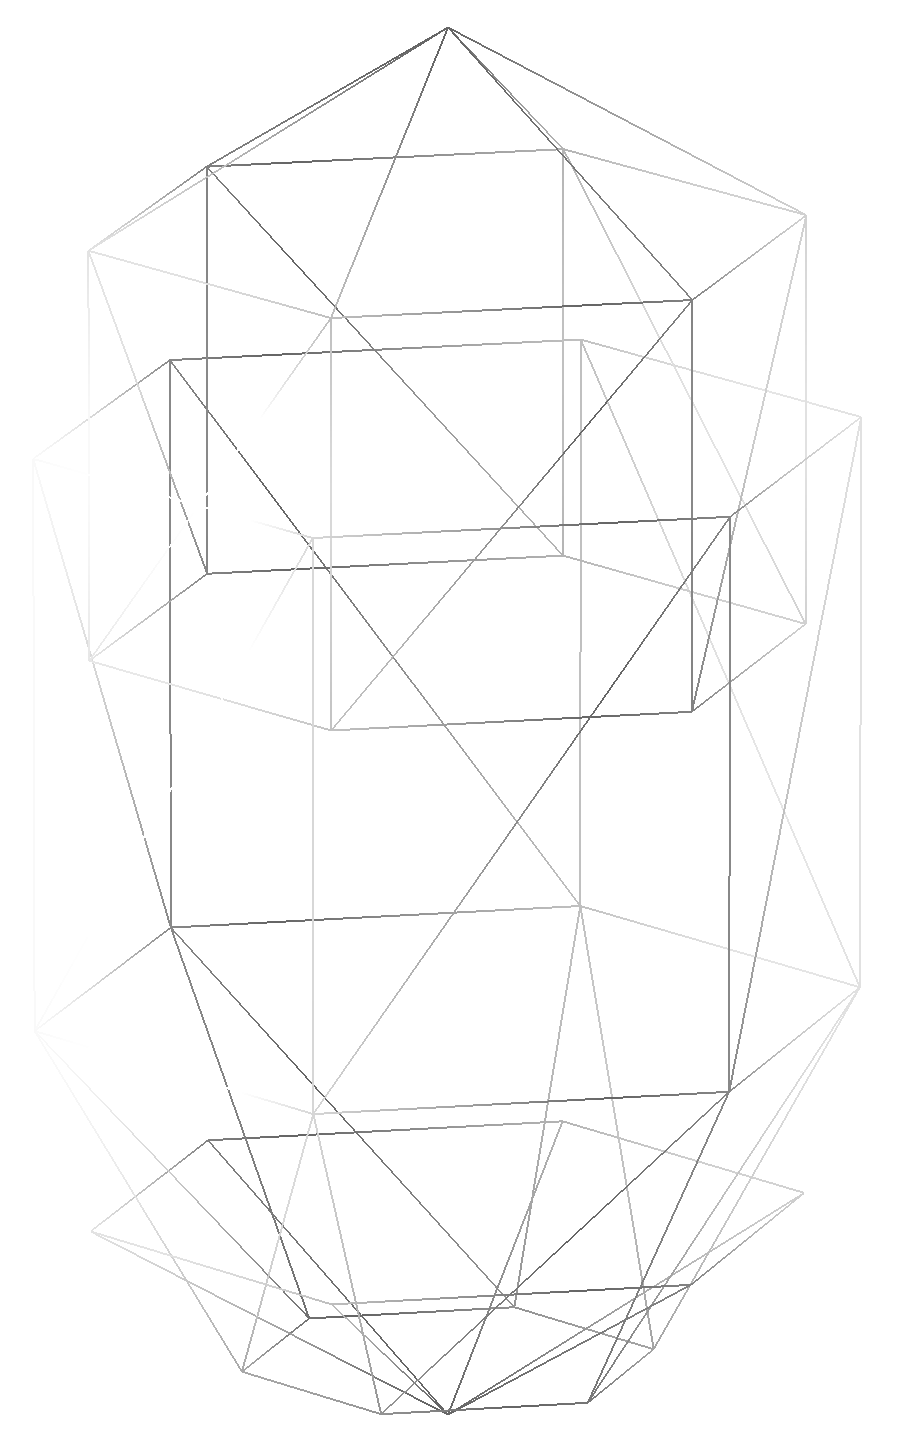
\includegraphics[width=\linewidth]{assets/images/shapes/bugold/bad_mesh_low_w}
    \caption{\makefirstuc{Low detail mesh}}
    \end{subfigure}
  \end{center}
  \caption{\makefirstuc{Bad spheocylinder mesh generated by WebMGA 2.0 with various mesh qualities.}}
  \label{fig:bad_spherocylinder_old}
\end{figure}
\begin{figure}
  \begin{center}
    \begin{subfigure}{0.2\textwidth}
    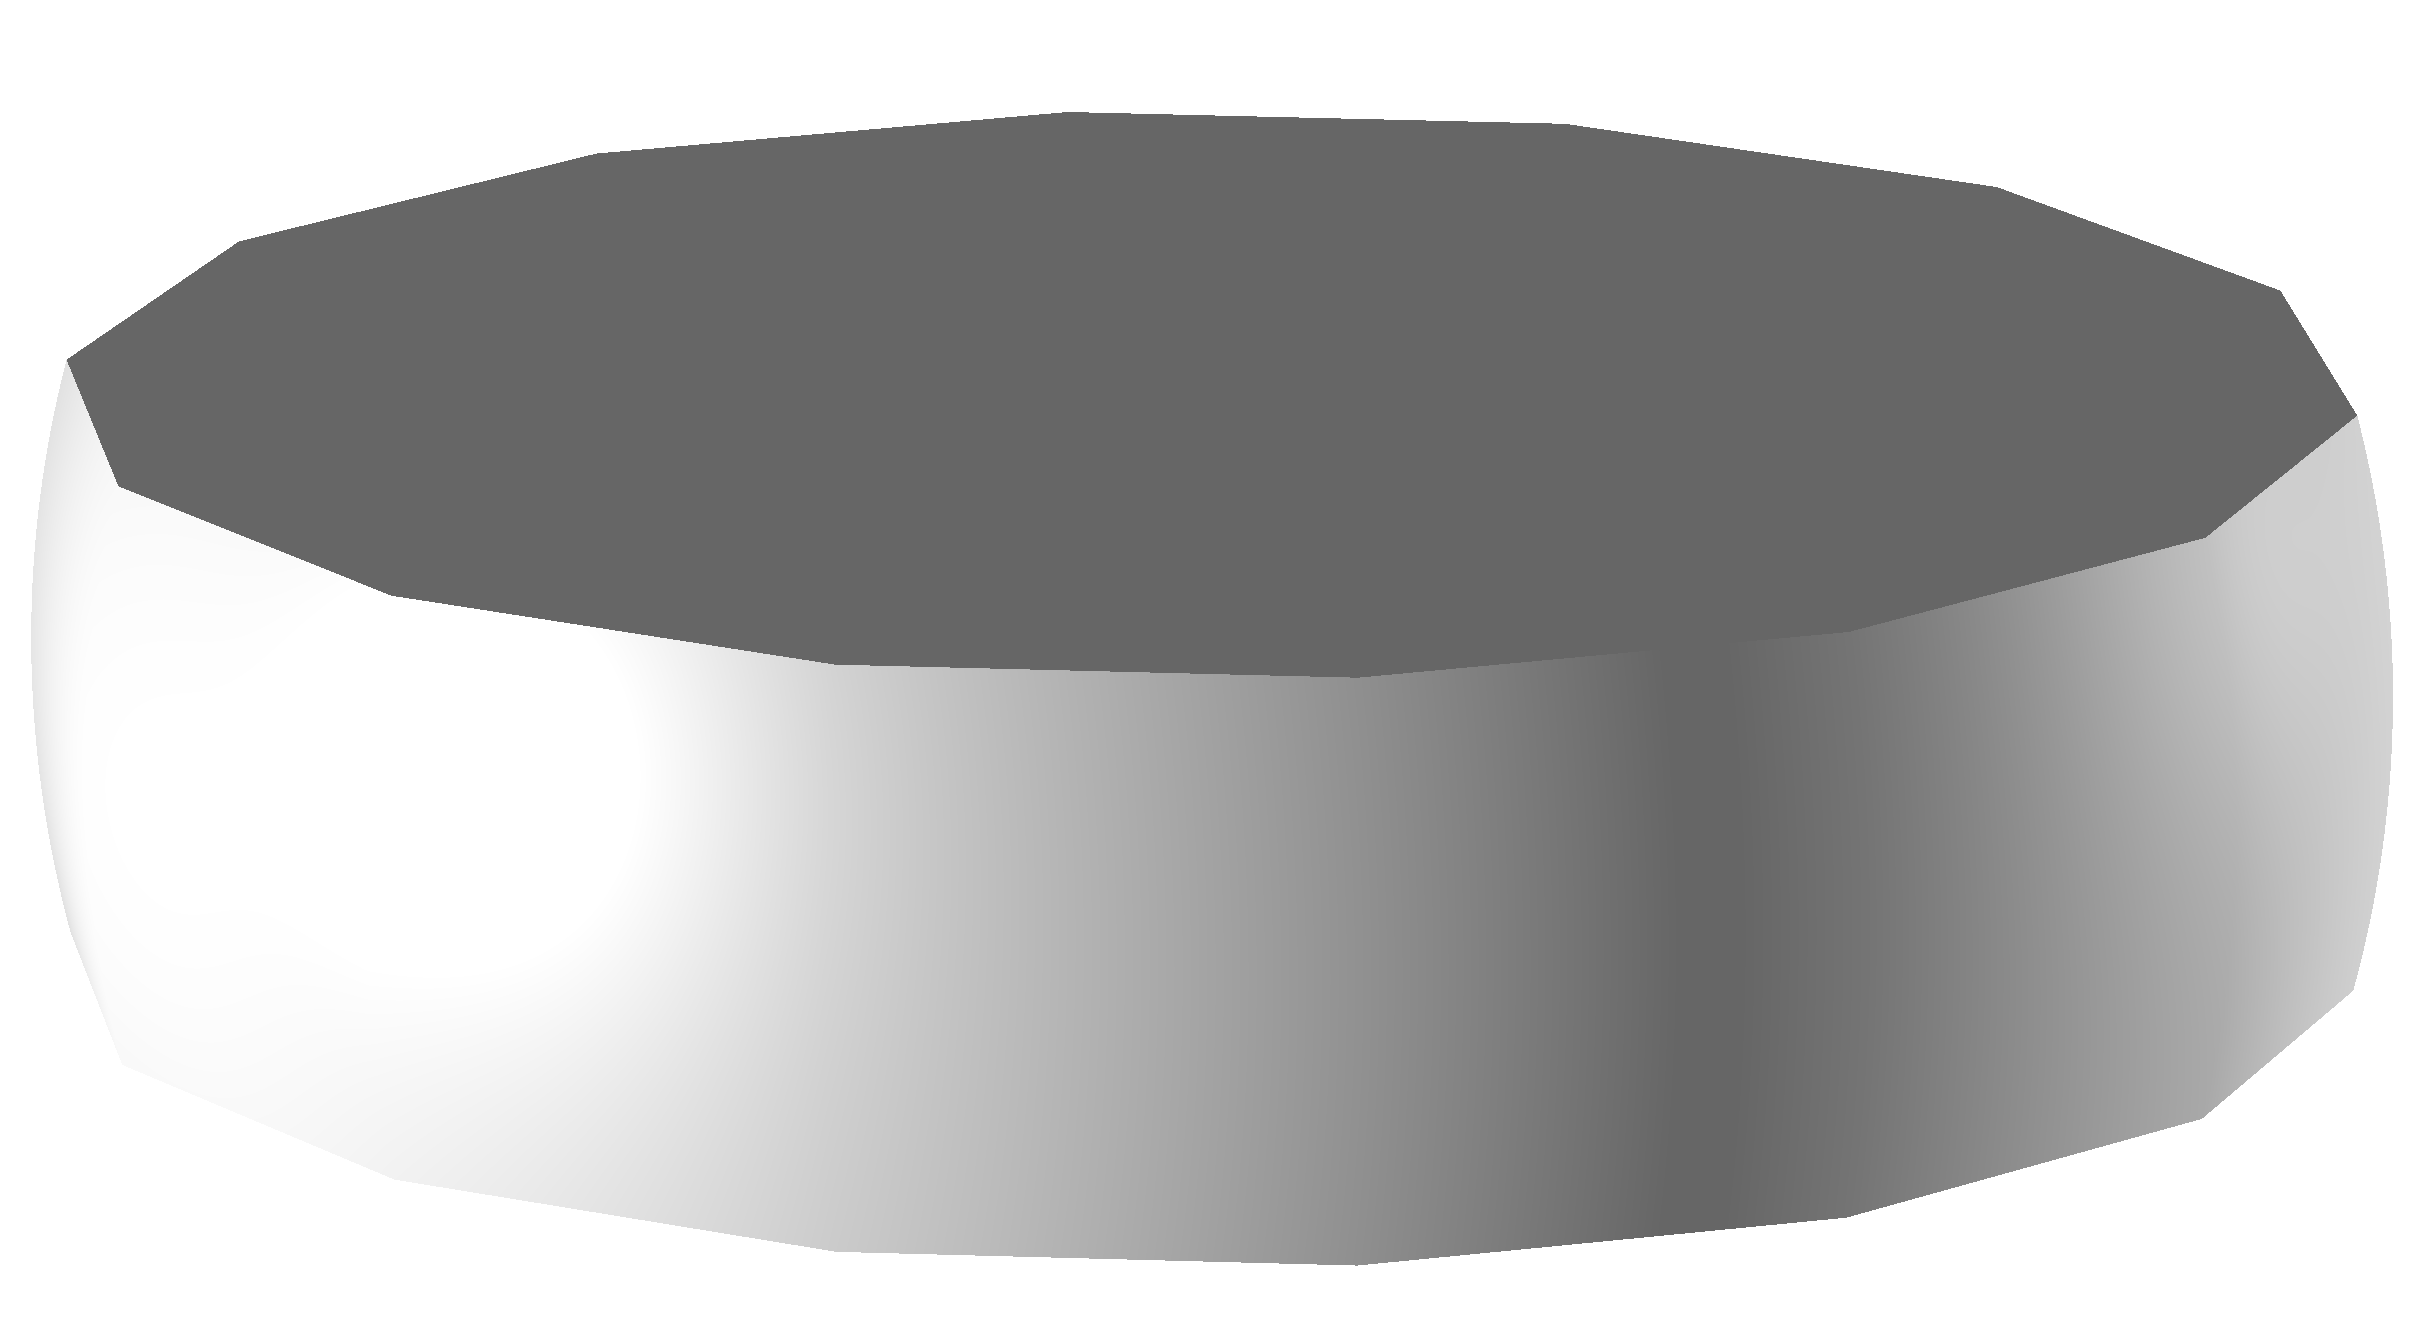
\includegraphics[width=\linewidth]{assets/images/shapes/bugold/scale_high}
    \caption{\makefirstuc{WebMGA 2.0}.}
    \end{subfigure}
      \begin{subfigure}{0.2\textwidth}
    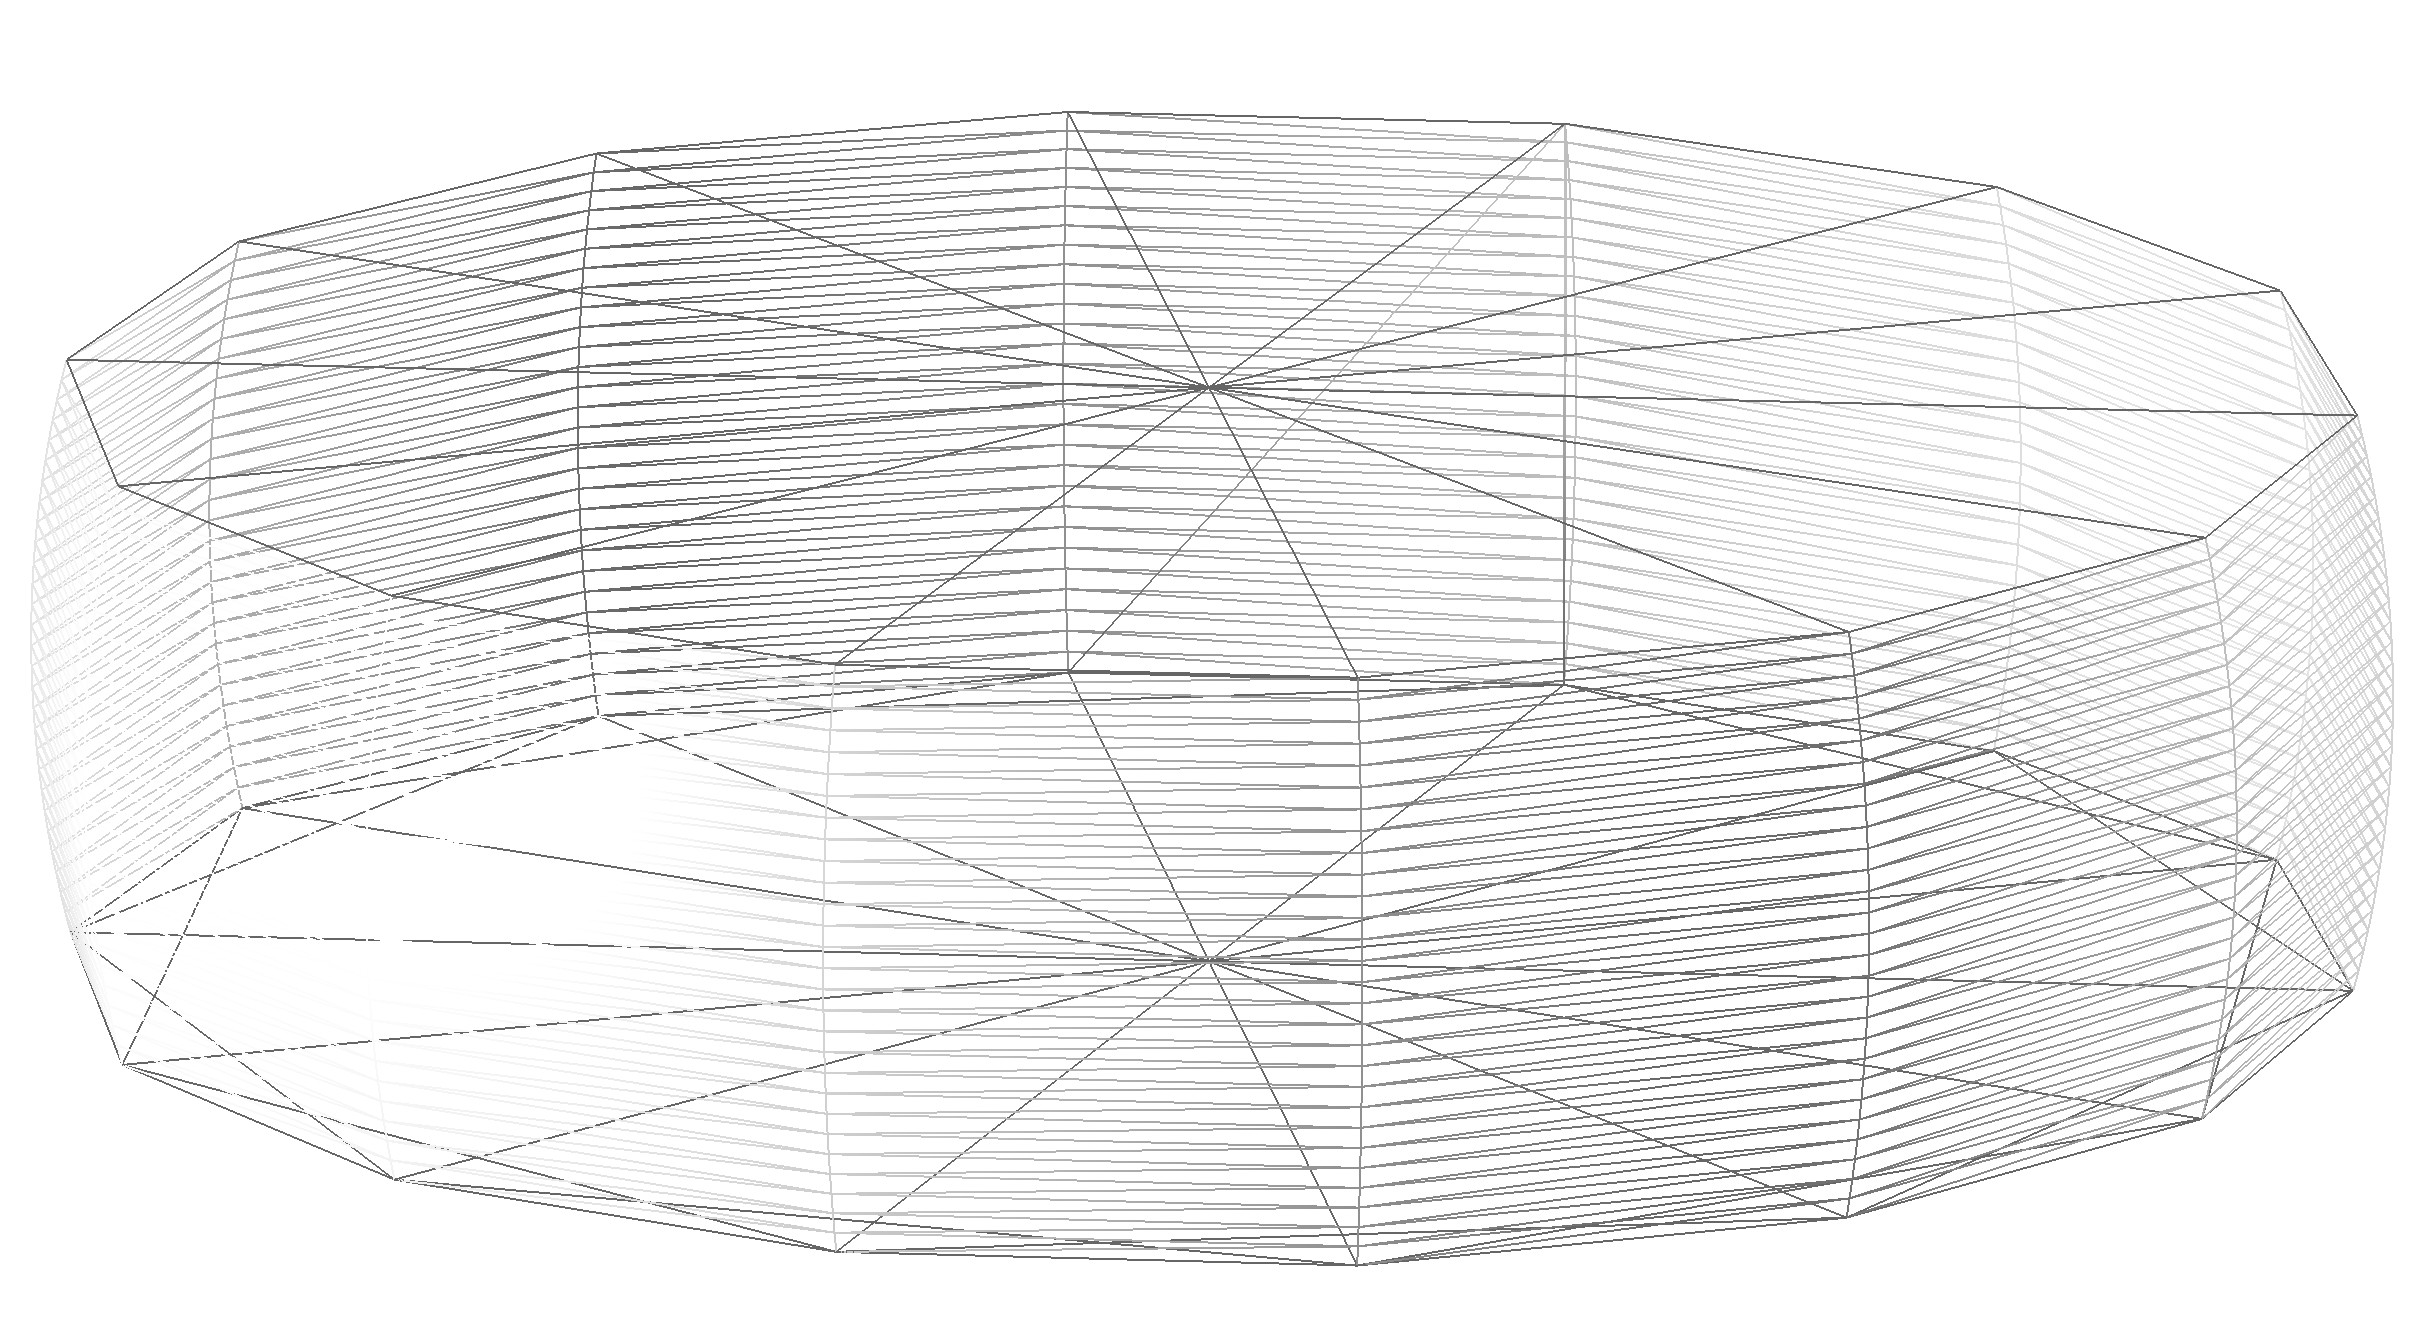
\includegraphics[width=\linewidth]{assets/images/shapes/bugold/scale_high_w}
    \caption{\makefirstuc{WebMGA 2.0}.}
    \end{subfigure}
    \begin{subfigure}{0.2\textwidth}
    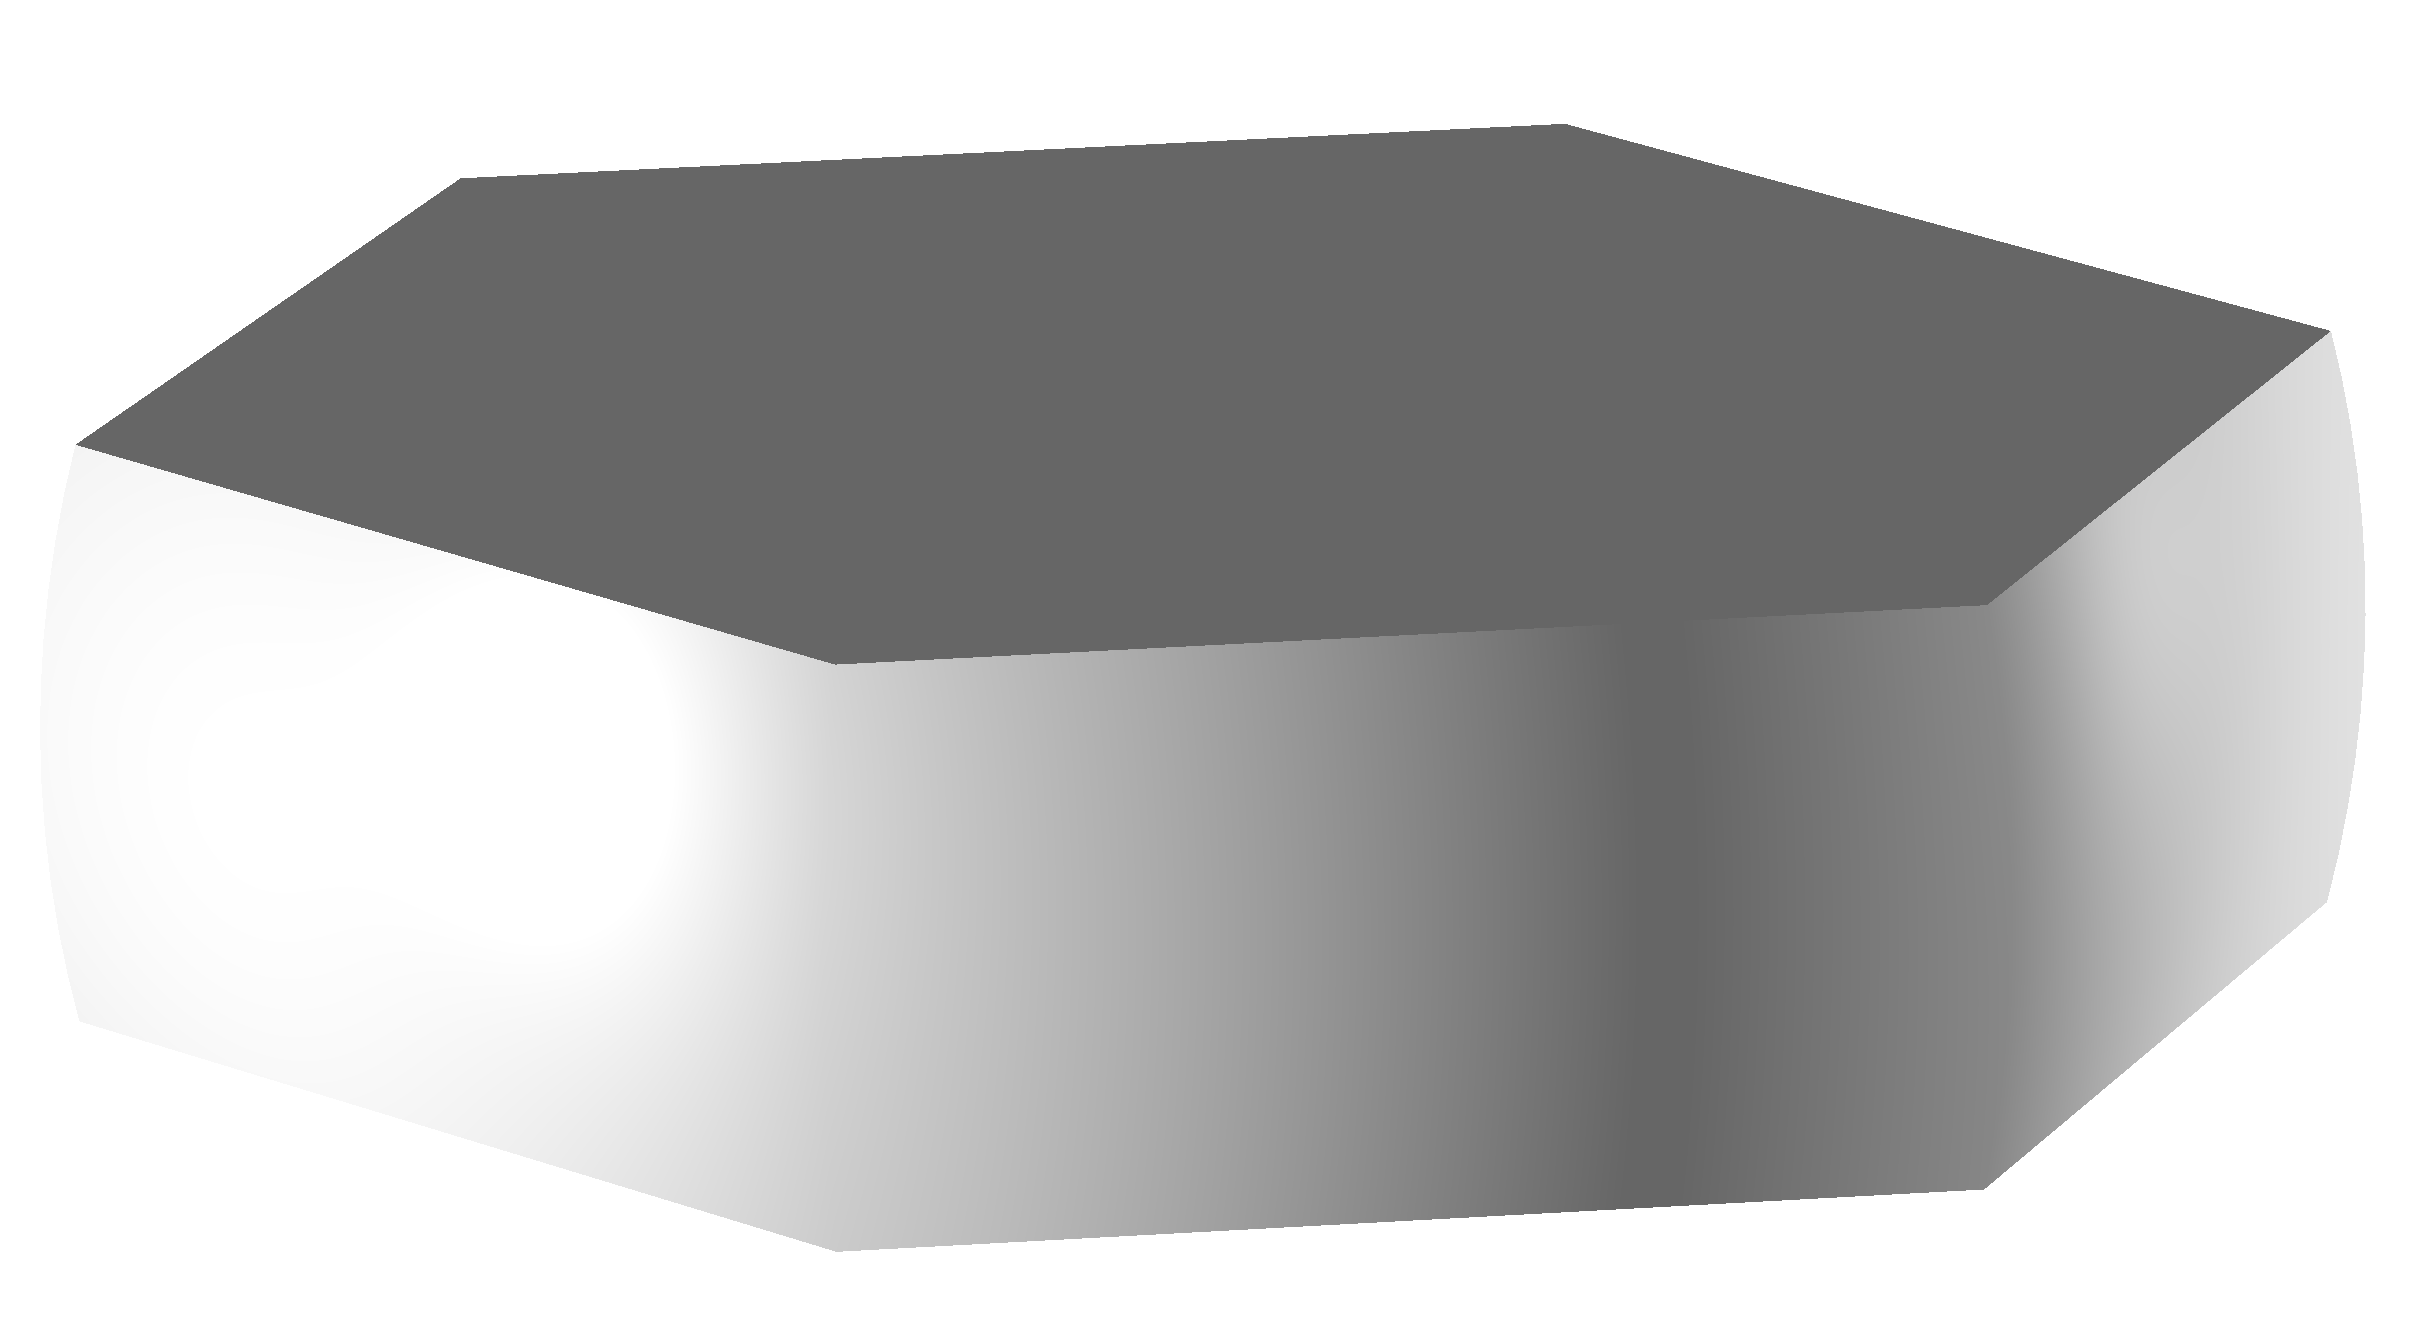
\includegraphics[width=\linewidth]{assets/images/shapes/bugold/scale_low}
    \caption{\makefirstuc{WebMGA 2.0}.}
    \end{subfigure}
    \begin{subfigure}{0.2\textwidth}
    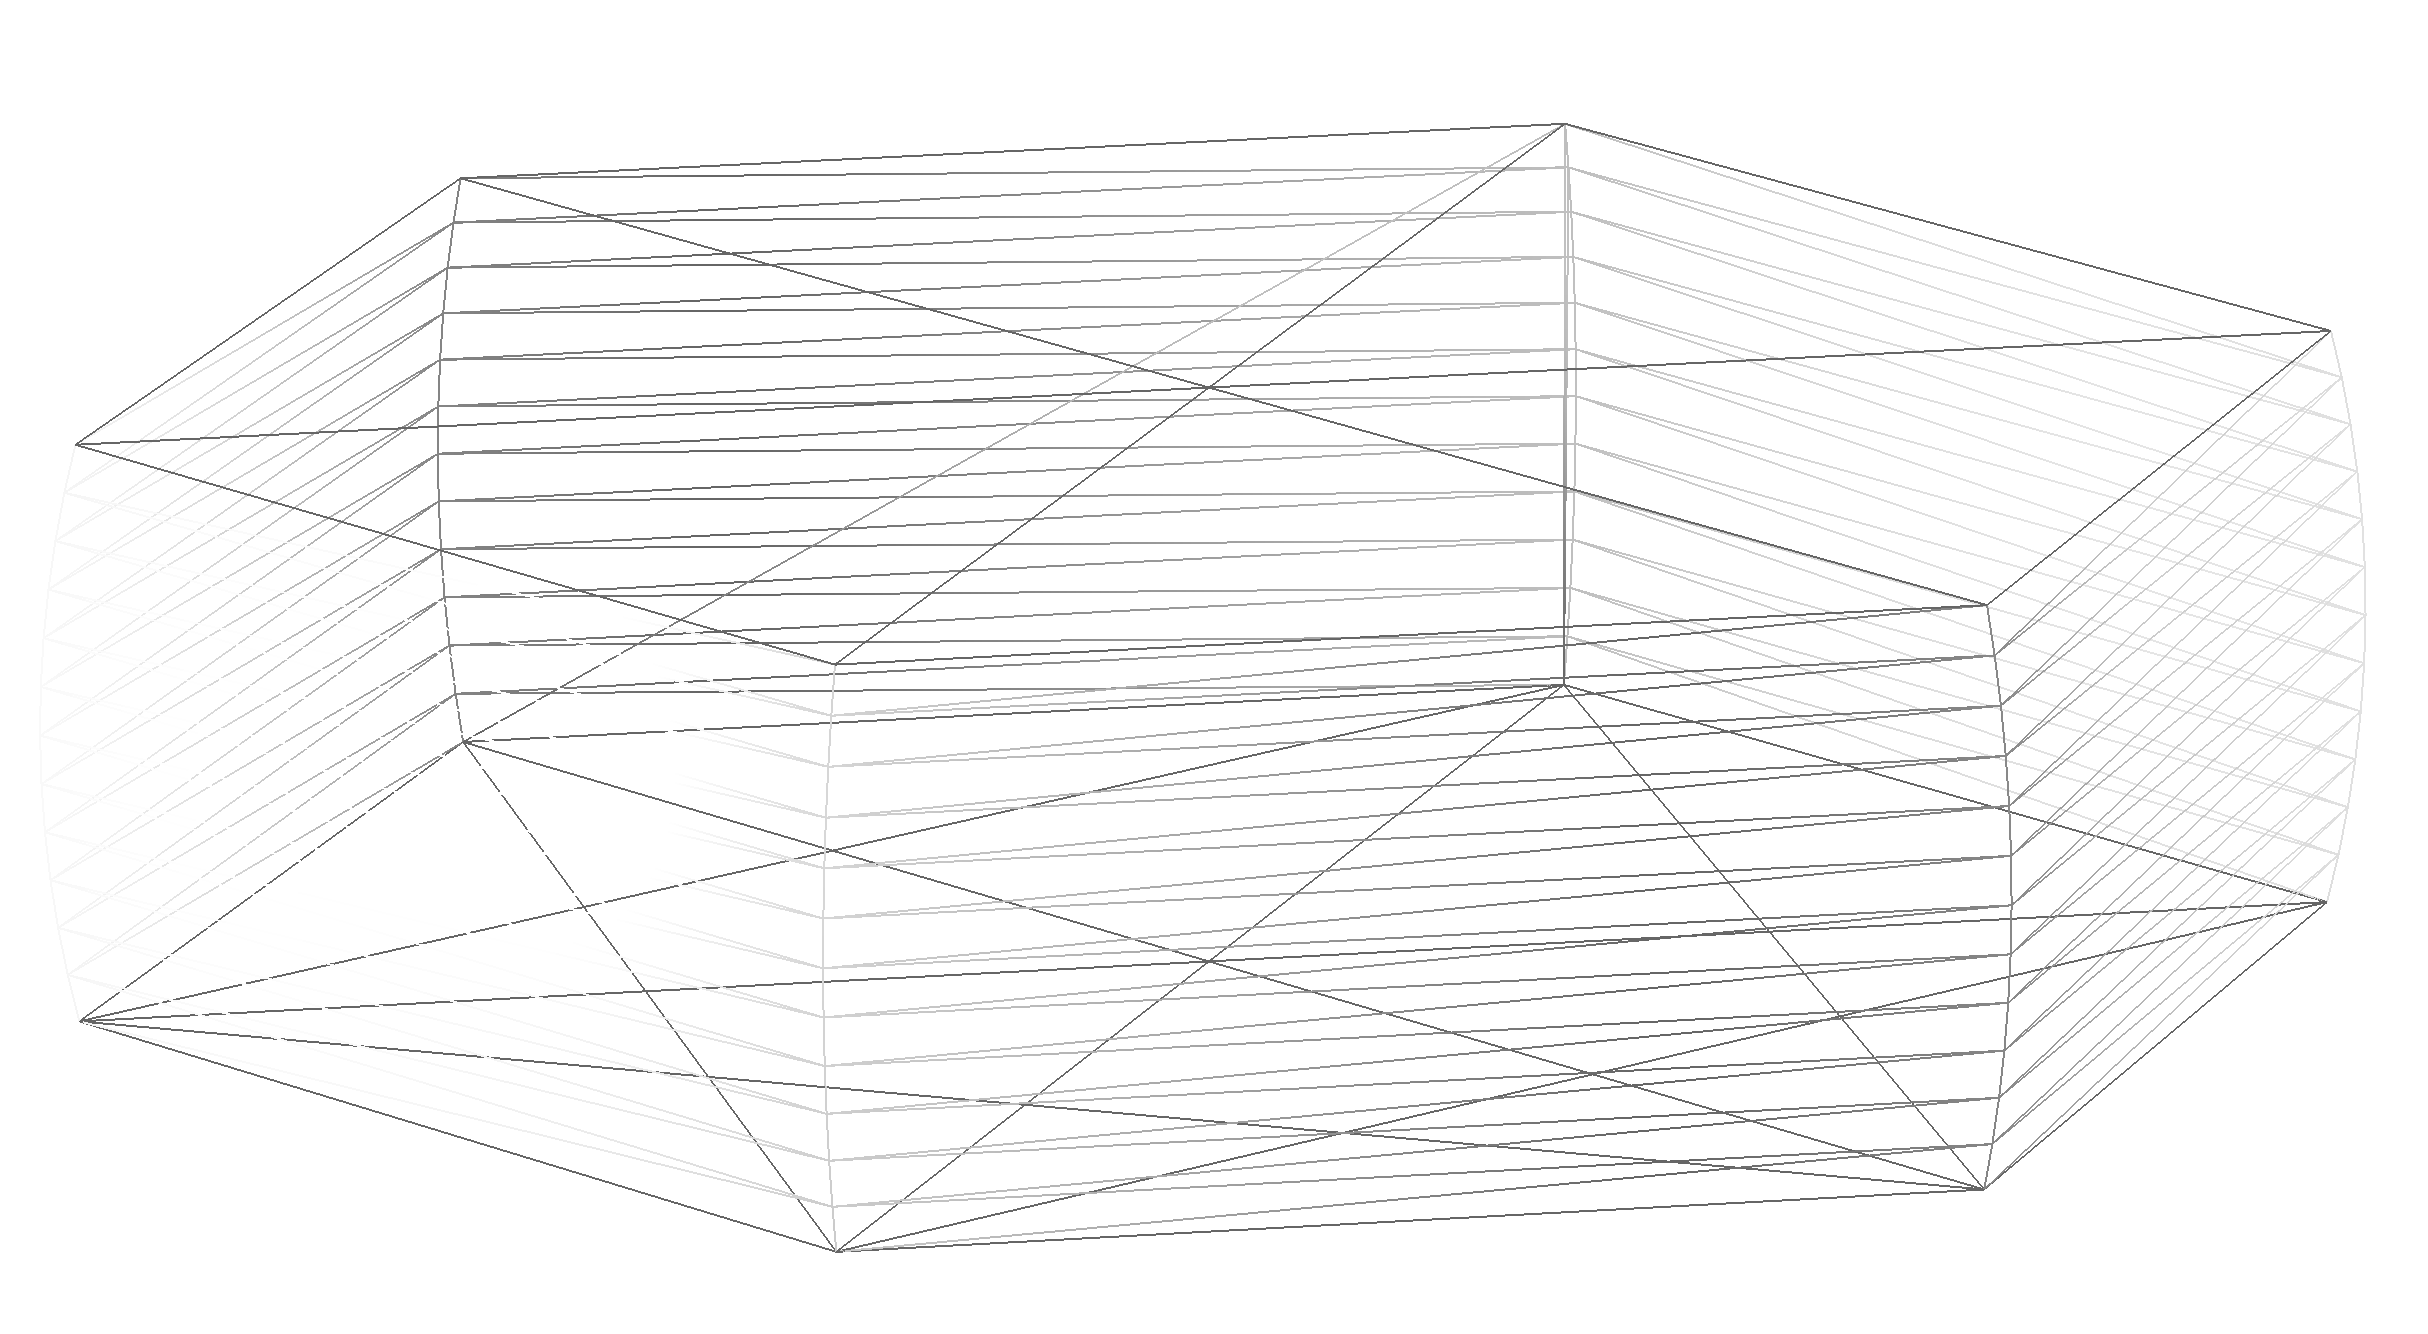
\includegraphics[width=\linewidth]{assets/images/shapes/bugold/scale_low_w}
    \caption{\makefirstuc{WebMGA 2.0}.}
    \end{subfigure}
  \end{center}
  \caption{\makefirstuc{Notably higher mesh quality vertically for double cut sphere with WebMGA 2.0}.}
  \label{fig:uneven_mesh_old}
\end{figure}
\begin{figure}
  \begin{center}
    \begin{subfigure}{0.4\textwidth}
    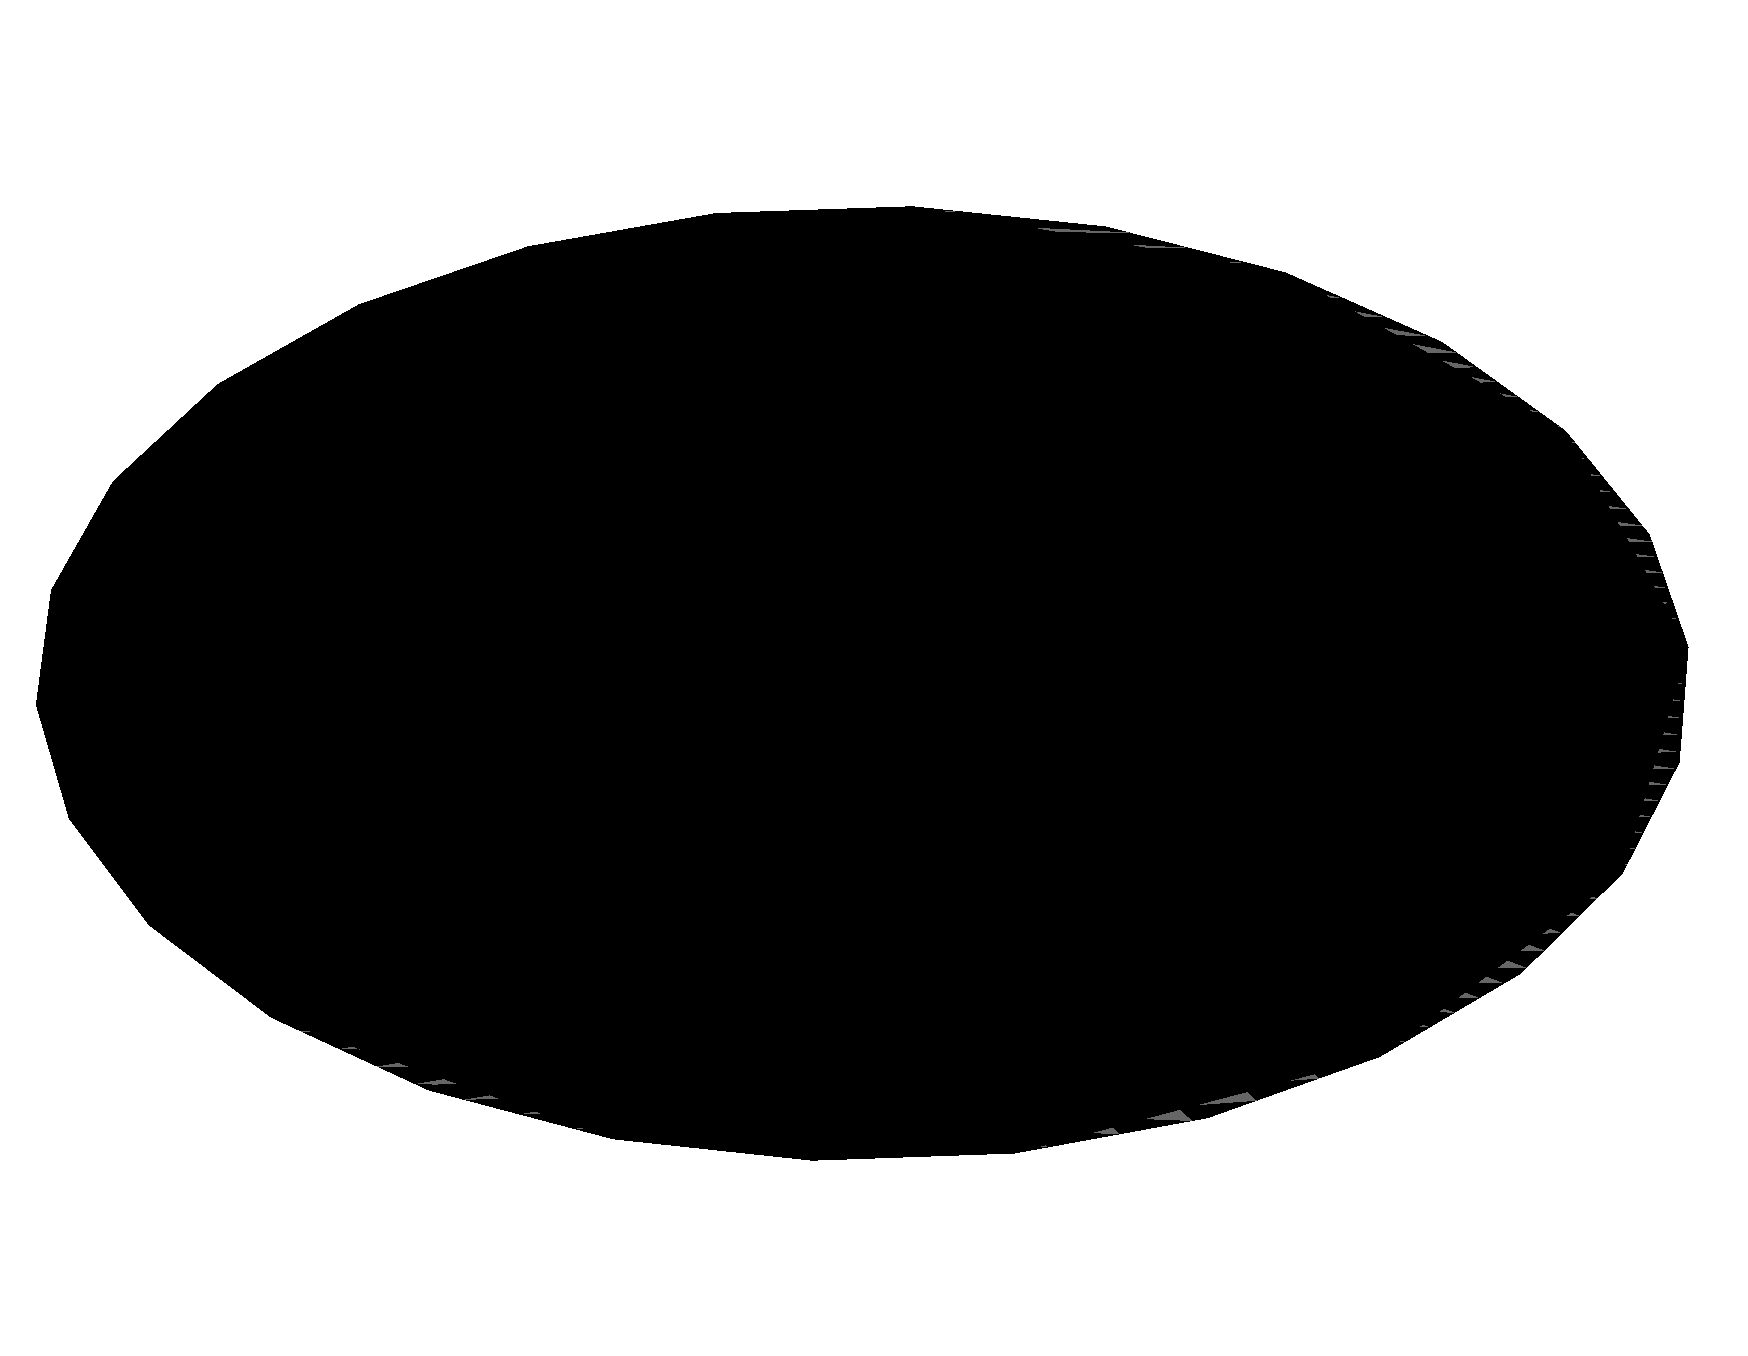
\includegraphics[width=\linewidth]{assets/images/shapes/bugold/no_height}
    \caption{\makefirstuc{WebMGA 2.0 Shape}.}
    \end{subfigure}
    \begin{subfigure}{0.4\textwidth}
    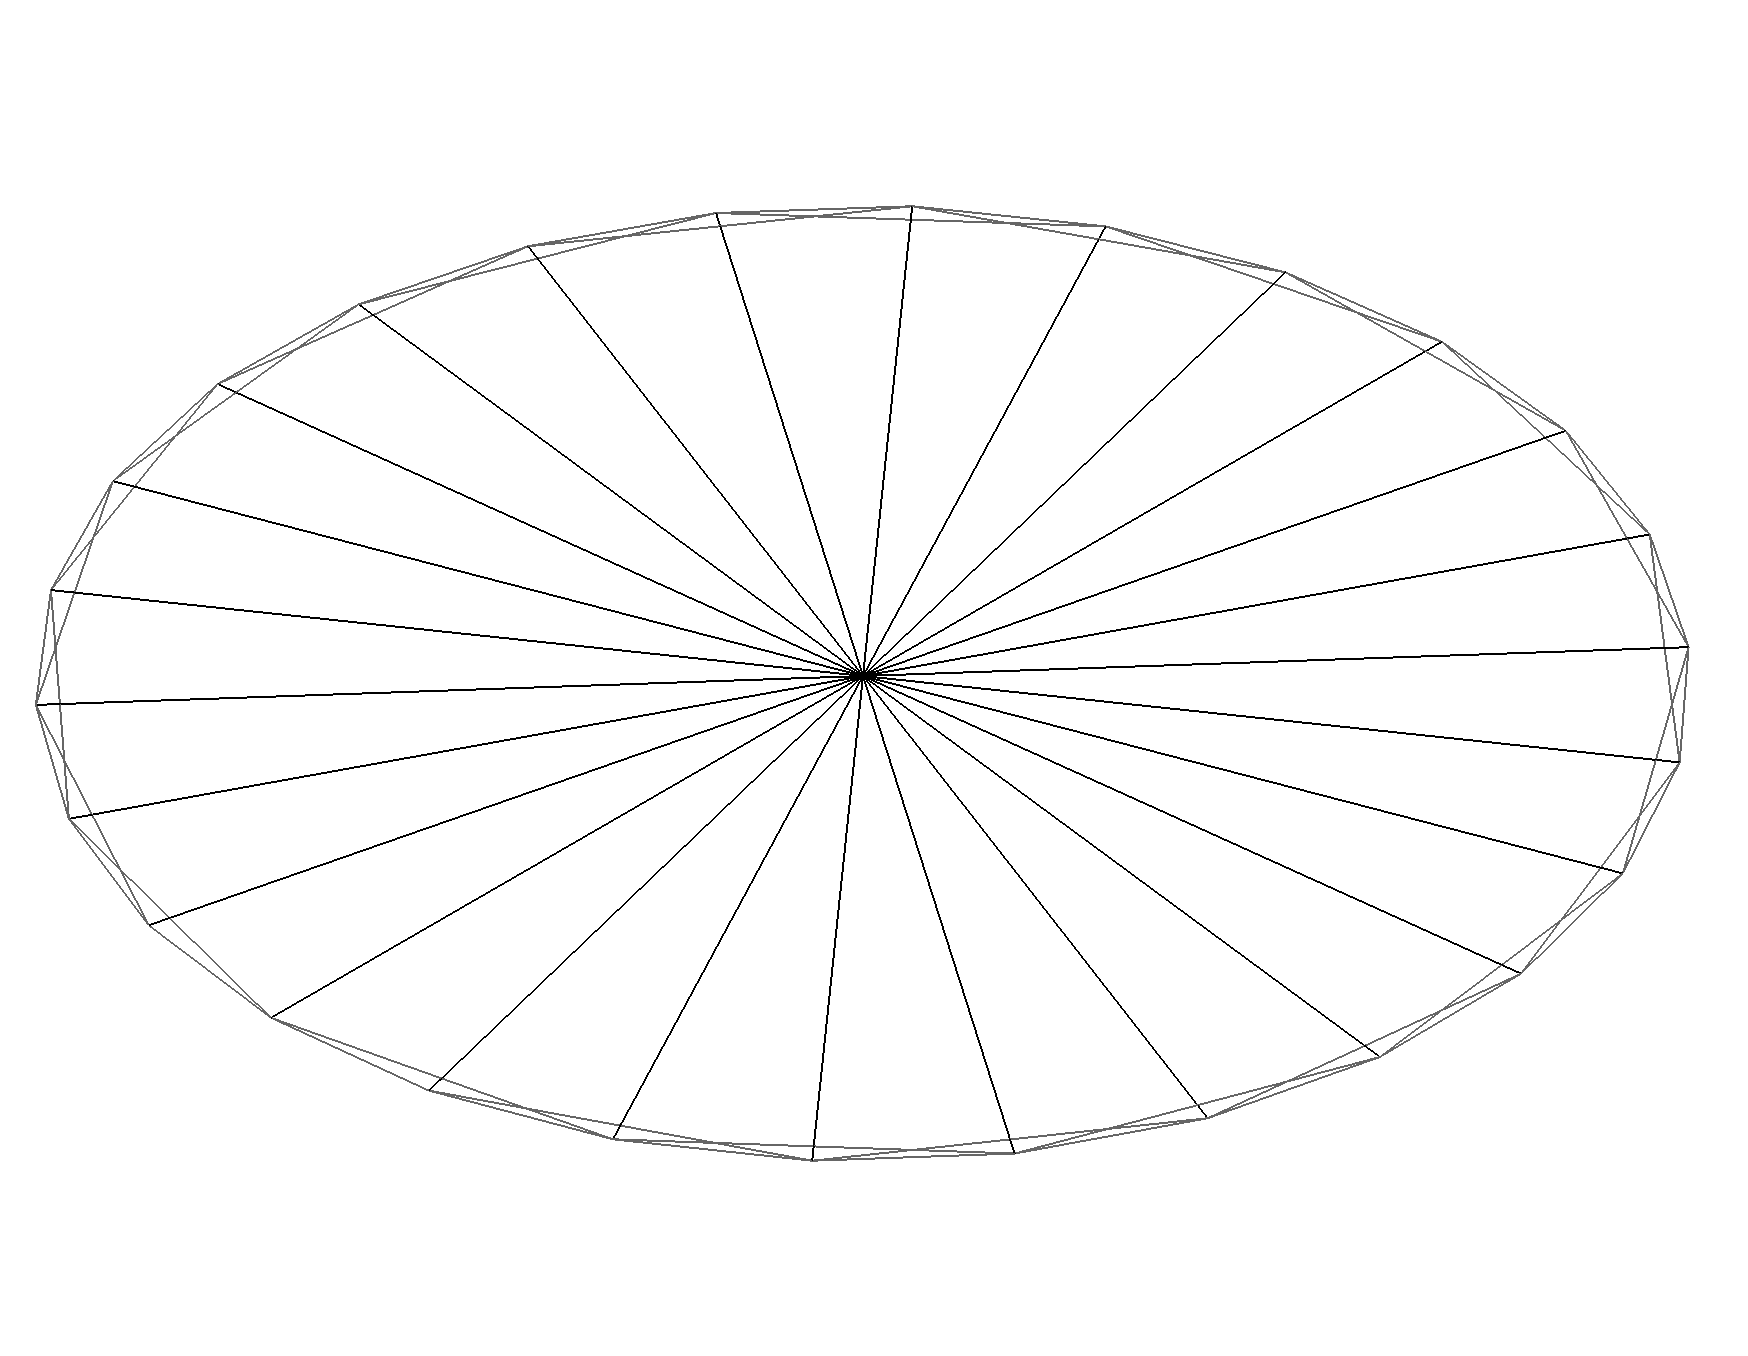
\includegraphics[width=\linewidth]{assets/images/shapes/bugold/no_height_w}
    \caption{\makefirstuc{WebMGA 2.0 Wireframe}.}
    \end{subfigure}
    \begin{subfigure}{0.4\textwidth}
    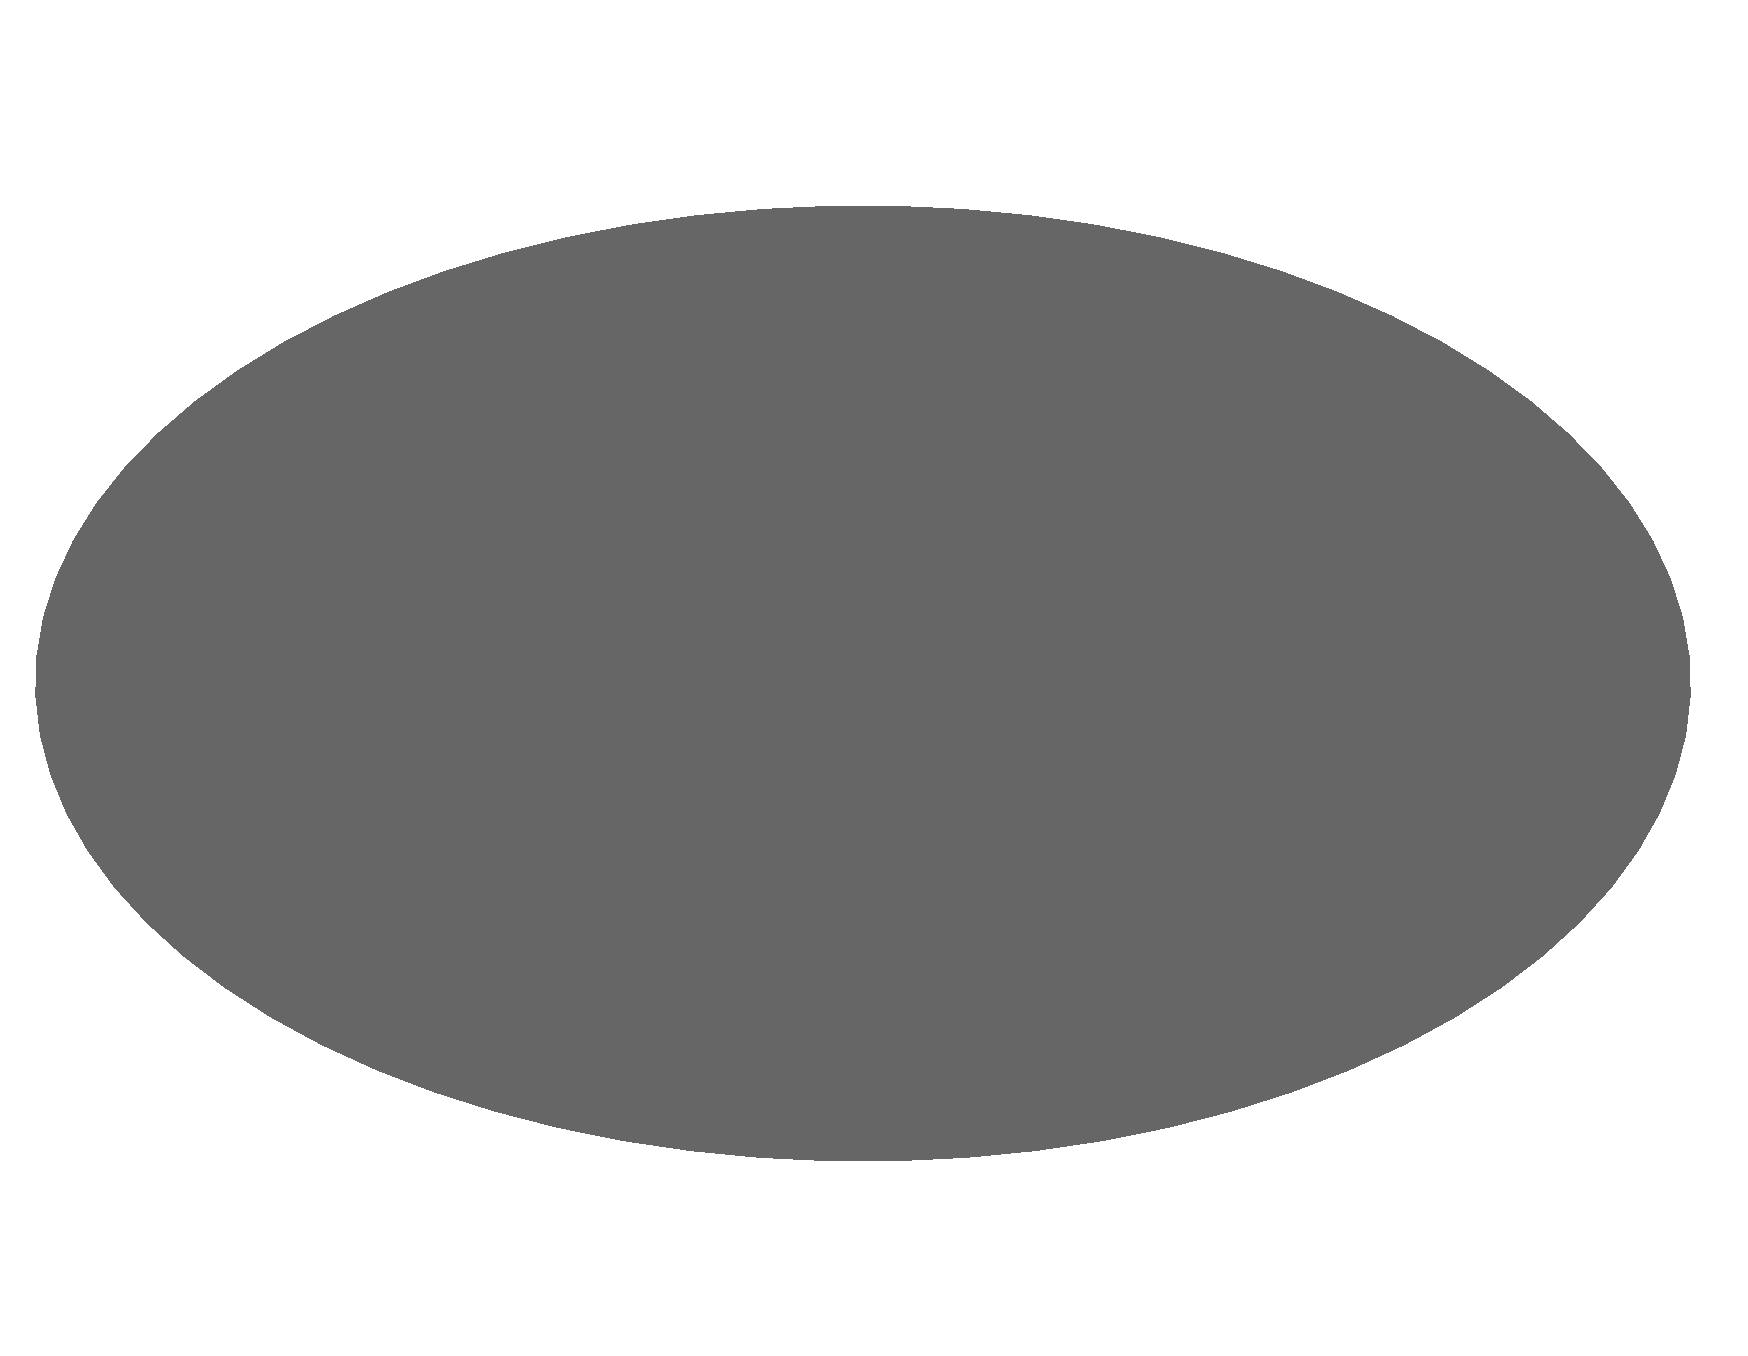
\includegraphics[width=\linewidth]{assets/images/shapes/bugnew/no_height}
    \caption{\makefirstuc{WebMGA 3.0 Shape}.}
    \end{subfigure}
    \begin{subfigure}{0.4\textwidth}
    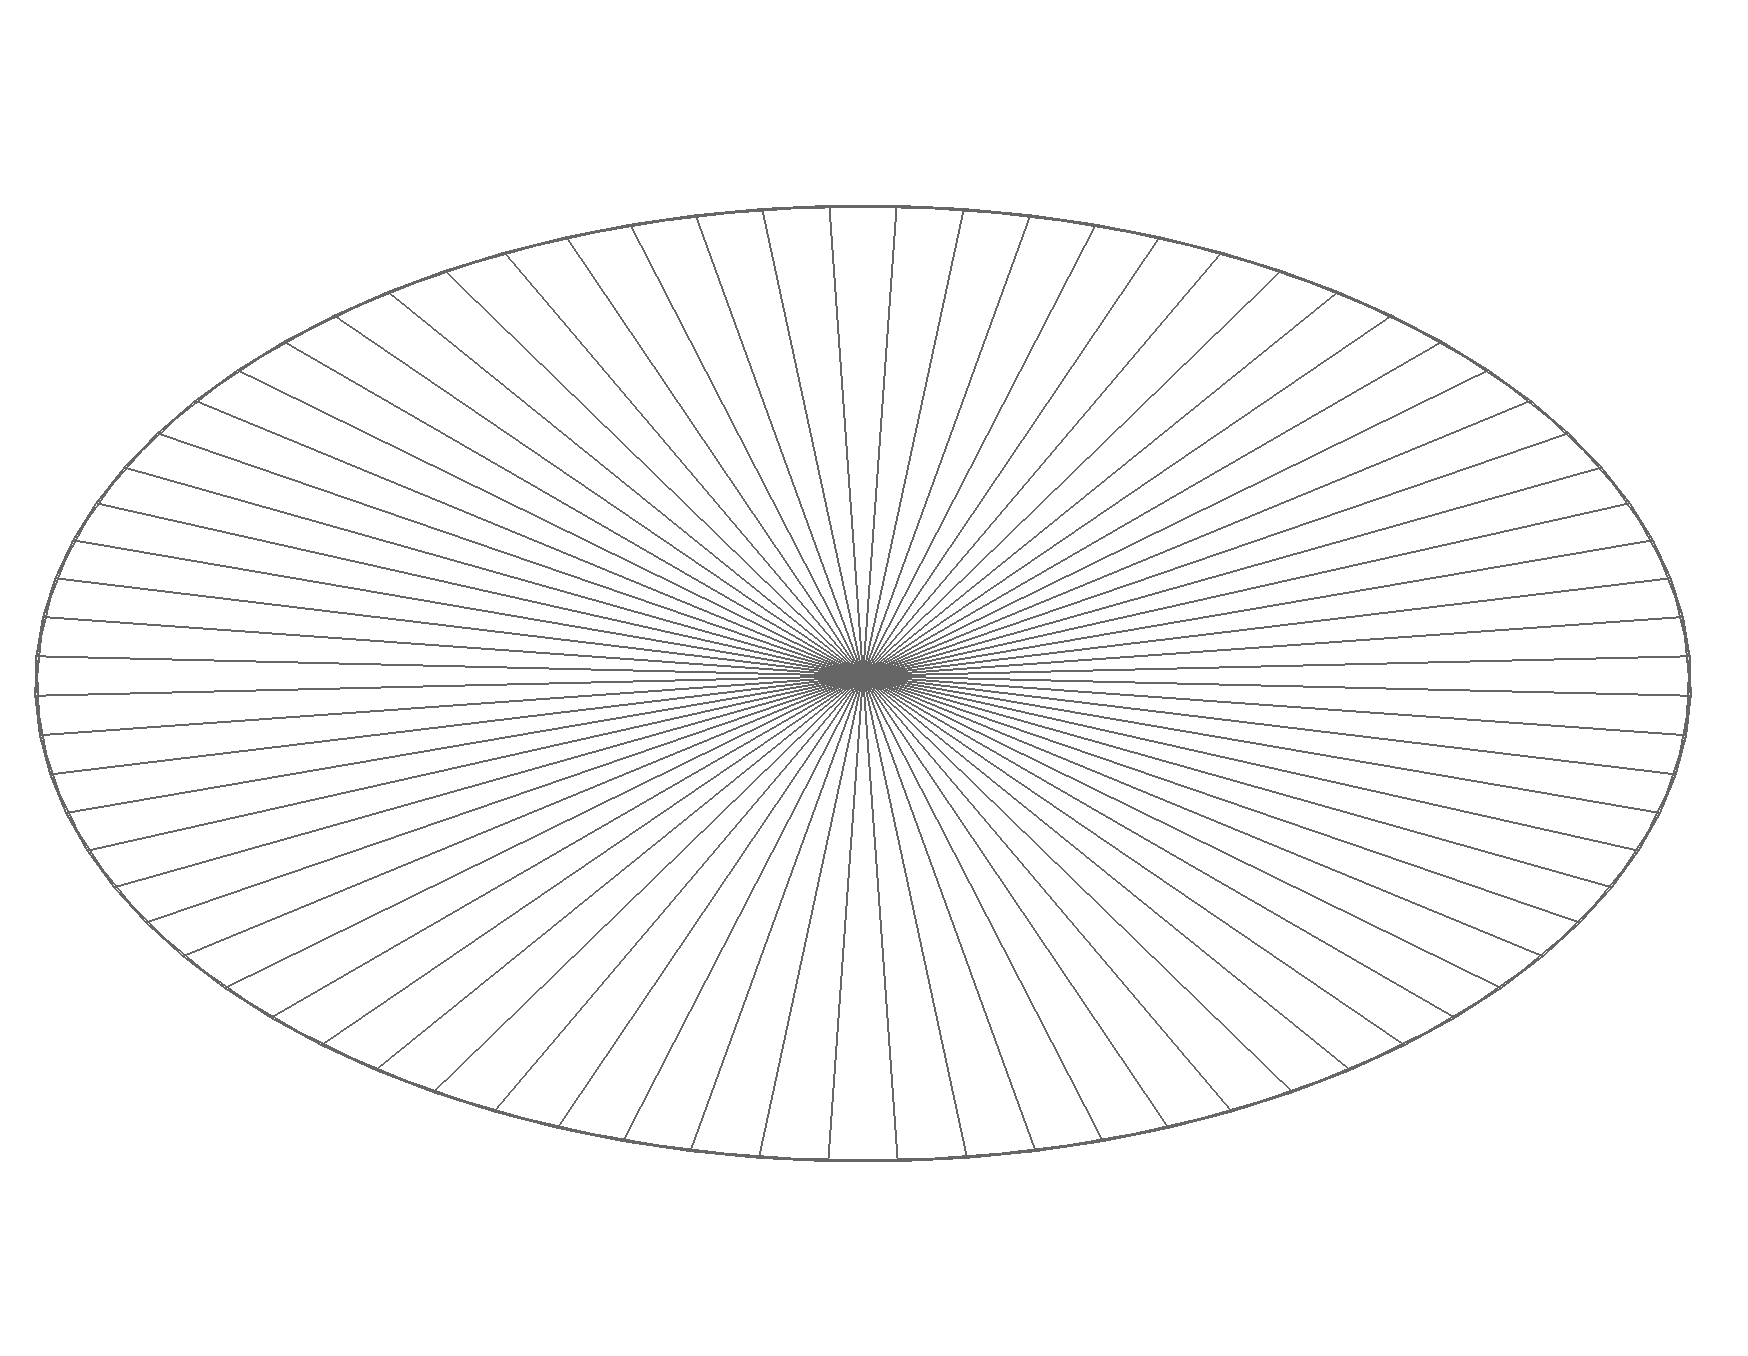
\includegraphics[width=\linewidth]{assets/images/shapes/bugnew/no_height_w}
    \caption{\makefirstuc{WebMGA 3.0 Wireframe}.}
    \end{subfigure}
  \end{center}
  \caption{\makefirstuc{Buggy shape representation when double cut sphere has 0 height}.}
  \label{fig:no_height_bug_old}
\end{figure}

\subsection{Improvement Goals}
\begin{itemize}
  \item Implement sphere generation
  \item Optimise existing shape generation using new sphere as base
    \begin{itemize}
      \item Ellipsoid
      \item Spherocylinder
      \item Spheroplatelet
      \item Double cut sphere
      \item New geometries should have well distributed vertices to address issue shown in \cref{fig:uneven_mesh_old}.
      \item Geometry meshes should have similar triangle counts and visual quality at equivalent LOD settings. This motivates reimplementation of existing shapes.
    \end{itemize}
  \item Implement new shapes
    \begin{itemize}
      \item Cut sphere
      \item Spherical cap
      \item Lens
      \item Biconvex lens
    \end{itemize}
    \item Recreate configuration in \cref{fig:cinacchi_lens}
          \begin{itemize}
      \item Implement Cinacchi lens parameterisation
    \end{itemize}
    \item Fix bugged spherocylinder mesh (\cref{fig:bad_spherocylinder_old})
    \item Fix double cut sphere 0 height bug (\cref{fig:no_height_bug_old})
\end{itemize}

\subsection{WebMGA 3.0 Implementation}
\subsubsection{Sphere}
\label{sphere_gen_sec}
Key to the new shape implementations is the implementation for the sphere (\cref{fig:sphere_shape}, parameter ``Radius''). The sphere mesh is generated by sampling points across the sphere's surface in such a way as to split it into a finite number of flat, triangular sub-faces as shown in \cref{fig:sphere_vertices}. This sampling is performed with the spherical coordinates system for some sphere radius $r$, azimuthal angles $\theta$, and polar angles $\phi$, converted to an equivalent Cartesian form. A point in spherical coordinate space is denoted $\mathbf{r}_\mathrm{s}$, while an identical point in Cartesian space is denoted $\mathbf{r}_\mathrm{C}$,

\begin{equation}
\mathbf{r}_\mathrm{s}=\begin{pmatrix}r\\\phi\\\theta\end{pmatrix}
\label{sphere_equation_spherical}
\end{equation}

\begin{equation}
\mathbf{r}_\mathrm{C}=\begin{pmatrix}r\sin\phi \cos\theta\\
r\sin\phi \sin\theta\\
r\cos\phi\end{pmatrix}.
\label{sphere_equation_cartesian}
\end{equation}

Any unique point on the origin centred $r$ sphere can be uniquely defined by some $(\theta,\phi)$ pair. Therefore, to evenly space points across the surface, a set of $\theta$s and $\phi$s is generated by taking $n$ (essentially a measure of mesh quality) evenly spaced values over the interval of a full circular rotation ($[0, 2\pi)$). Each unique pairing $(\phi,\gamma)$, along with $r$, is used to produce the full set of Cartesian vertices using \cref{sphere_equation_cartesian}. This method is sufficient to produce a sphere mesh as in \cref{fig:old_sphere} from WebMGA 2.0. The sampling is modified slightly for WebMGA 3.0 to produce a mesh as in \cref{fig:new_sphere} by offsetting each row such that points on one row lie half way between a pair of points on the row above since it produces a slightly more visually satisfying mesh. The code was rewritten from scratch since most other shapes result from slight modifications to the sphere generation process, and the initial WebMGA 2.0 implementation was over-complicated and proved difficult to extend.

\paragraph{Vertex Ordering:} Since WebMGA 2.0 implements the back face culling optimisation\cite{face_cull} for mesh triangles, during the triangle generation process it must be ensured that vertices are arranged correctly to ensure the front face is on the exterior of the shape. When back face culling is used, the renderer will only shade triangles which it believes are facing towards the camera, and skip this for triangles facing away. The direction a triangle faces is defined by its winding. The two possible windings are shown in \cref{fig:triangle}. To ensure the triangle winding is correct during sphere generation, the vertex rows and columns are arranged such that, using the numbering from \cref{fig:triangle}, if vertex 1 is at index $i$ on row $j$, then vertex 2 and 3 will be placed at indexes $i$ and $i+1$ on row $j+1$. When triangles are defined, they can be read from the vertex array in this order as appropriate.

\begin{figure}
  \begin{center}
    \begin{subfigure}{0.4\textwidth}
      \includesvg[width=\textwidth]{assets/images/shape_diagrams/tri_1}
      \caption{Normal faces out of screen.}
      \label{fig:out_normal}
    \end{subfigure}
        \begin{subfigure}{0.4\textwidth}
      \includesvg[width=\textwidth]{assets/images/shape_diagrams/tri_2}
      \caption{Normal faces into screen.}
      \label{fig:in_normal}
    \end{subfigure}
  \end{center}
  \caption{Triangle vertex ordering effect on normal direction (using right hand rule).}
  \label{fig:triangle}
\end{figure}

\paragraph{Optimisation:} \label{sphere_optim}Some optimisations are implemented to efficiently generate a full set of vertices while sampling only $\frac{1}{4}$ of the points around the sphere's surface. This uses the fact that the origin centred sphere is symmetrical in each of the $xy$, $xz$, and $yz$ planes. Points for the quarter sphere can be generated by applying \cref{sphere_equation_cartesian} with all pairings of $\frac{n}{2}$ evenly spaced $\theta \in [0, \pi)$, and $\frac{n}{2}$ evenly spaced $\phi \in [0, \frac{\pi}{2}]$. These points are arranged in a 3d array corresponding to rows (from $\phi$) and columns (from $\theta$).

An additional set of points for the another quarter of the top hemisphere is trivially generated  by copying the original quarter vertices and negating the $x$ and $y$ values. The bottom hemisphere is generated by duplicating the top hemisphere and negating the $z$ values. Concatenating the top and bottom hemisphere arrays results in a full sphere, however with an incorrect vertex order to correctly connect the vertices. To fix this, the bottom hemisphere array must first be reversed (i.e. reverse row order), and each row should have its components shifted such that the top row of vertices correctly aligns with the bottom row of vertices for the top hemisphere.

\begin{figure}
  \begin{center}
    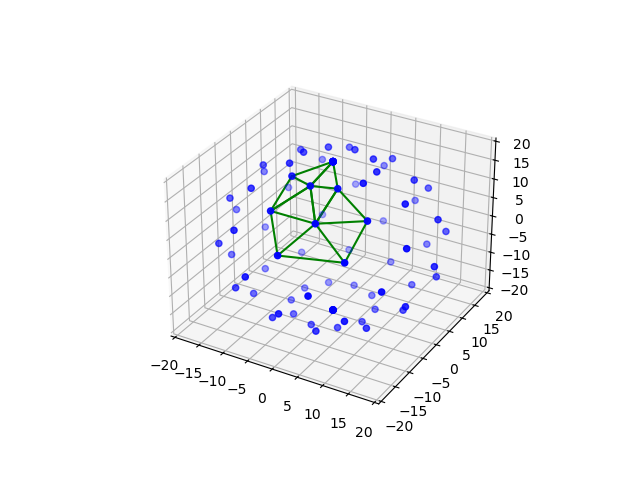
\includegraphics[width=0.8\linewidth]{assets/images/shapes/sphere_vertices}
    \caption{Example sphere vertex distribution ($9\times10$ vertical$\times$horizontal samples). Some mesh edges shown to demonstrate mesh construction from vertices.}
    \label{fig:sphere_vertices}
  \end{center}
\end{figure}

\shapefigure{sphere}{sphere}

\subsubsection{Ellipsoid}
The ellipsoid shape (\cref{fig:ellipsoid_shape}, parameters ``X'', ``Y'', ``Z'') can be represented as an origin centred sphere of radius 1 scaled in the $x$, $y$ and $z$ directions by some scalar value in each direction. This can be represented by a slightly modified form of the Cartesian sphere equation in \cref{sphere_equation_cartesian}, where $\mathbf{S}$ denotes some scaling vector,
\begin{equation}
\mathbf{r}_\mathrm{e}=\begin{pmatrix}s_x r\sin\phi \cos\theta\\
s_y r\sin\phi \sin\theta\\
s_z r\cos\theta\end{pmatrix}
=\mathbf{S} \odot \mathbf{r}_\mathrm{C}.
\label{ellipsoid_equation}
\end{equation}
From this formulation, it can be seen that an ellipsoid can be generated by slightly modifying the vertex sampling process for a sphere, whilst leaving the rest of the mesh building process unchanged. A sphere point can be sampled using \cref{sphere_equation_cartesian} with radius 1 and then multiplied by the scaling vector $\begin{pmatrix}s_x,s_y,s_z\end{pmatrix}^\mathsf{T}$ to give an equivalent result to \cref{ellipsoid_equation}.

In the program this is implemented by creating an ``Ellipsoid'' class as a child of the ``Sphere'' class and overriding the ``sample\_sphere()'' method. Since this implementation is so simple, the JavaScript code is provided below:

\begin{adjustbox}{width=\textwidth}
\begin{lstlisting}
//Ellipsoid mesh generator
export class Ellipsoid extends Sphere {
    //Scale factor in [x, y, z] directions
    scale: number[];

    constructor(x: number, y: number, z: number) {
        //Derive from origin centred sphere of radius 1
        super(1);
        this.scale = [x, y, z];
    }

    //Samples from ellipsoid instead of sphere
    sample_sphere(radius: number, theta: number, phi: number): number[] {
        //Multiply origin centred sphere coordinates by scale vector
        return math.dotMultiply(super.sample_sphere(radius, theta, phi), this.scale);
    }
}
\end{lstlisting}
\end{adjustbox}
\shapefigure{ellipsoid}{ellipsoid}

\subsubsection{Spheroplatelet}
The spheroplatelet shape (\cref{fig:spheroplatelet_shape}, parameters ``RadSphere'' and ``RadCircle'') is generated by modifying a generated sphere mesh. Vertices are iterated over and pushed outwards by applying the below formula, following on from \cref{sphere_equation_cartesian} with $c$ representing ``RadCircle'', $\mathbf{n}$ representing the sphere vertex normal in the $x,y$ plane, and $\mathbf{r}_\mathrm{p}$ representing a vertex coordinate,
\begin{equation}
\mathbf{n}=\begin{pmatrix}
  r_x\\
  r_y
\end{pmatrix}
\end{equation}
\begin{equation}
\mathbf{r}_\mathrm{p}=\mathbf{r}_\mathrm{C} + \frac{c\mathbf{n}}{\|\mathbf{n}\|_2}.
\end{equation}

This will leave an empty circle of points at the top and bottom of the transformed geometry which can be filled by generating an vertex at the top and bottom respectively by averaging the coordinates for each vertex on the corresponding circle's edge, splitting it into triangles. This can be observed on \cref{fig:new_spheroplatelet_w}.
\shapefigure{spheroplatelet}{spheroplatelet}

\subsubsection{Cut Sphere}
\label{cut_sphere_section}
\begin{figure}
  \begin{center}
    \begin{subfigure}{0.3\textwidth}
      \includesvg[width=\textwidth]{assets/images/shape_diagrams/cut_sphere}
      \caption{Cut sphere.}
      \label{fig:cut_sphere_diagram}
    \end{subfigure}
    \begin{subfigure}{0.3\textwidth}
      \includesvg[width=\textwidth]{assets/images/shape_diagrams/doublecut}
      \caption{Double cut sphere.}
      \label{fig:double_cut_diagram}
    \end{subfigure}
    \begin{subfigure}{0.3\textwidth}
      \includesvg[width=\textwidth]{assets/images/shape_diagrams/cap}
      \caption{Cap.}
      \label{fig:cap_diagram}
    \end{subfigure}
  \end{center}
  \caption{Cap and cut sphere shape diagrams. Lens outlines are shown by a red line, black lines demonstrate construction. Diagrams implemented by author using draw.io \cite{drawio}.}
  \label{fig:cap_cut_descriptions}
\end{figure}
The cut sphere shape (\cref{fig:cutsphere_shape}, parameters ``Radius'', ``zCut'') is implemented simply by sampling the sphere as before but over a reduced range of $\phi$ values. Since the sphere will not be completed, an empty circular face is left which can be filled by generating an additional vertex by averaging the coordinates for each vertex on the circle's edge, splitting it into triangles. This can be observed on \cref{fig:new_cutsphere_w}.

A cut sphere is parameterised in WebMGA using a parent sphere radius and a zCut distance. These are shown in \cref{fig:cut_sphere_diagram}, with characters $r$ and $x$ respectively. The new range of $\phi$s can be seen in the diagram as the range $[\alpha,\pi)$, which can be reinterpreted in terms of $r$ and $x$ as follows,
\begin{equation}
\alpha=\arcsin\frac{c}{r}
\end{equation}
\begin{equation}
c=\sqrt{r^2-x^2}
\end{equation}
\begin{equation}
[\alpha,\pi)=\left[\arcsin\frac{c}{r},\pi\right).
\end{equation}

\newshapefigure{cutsphere}{cut sphere}

\subsubsection{Double Cut Sphere}
The double cut sphere shape (\cref{fig:doublecutsphere_shape}, parameters ``Radius'', ``zCut'') is implemented simply by sampling the sphere as before but over a reduced range of $\phi$ values. Since the sphere will not be completed, two empty circular faces are left which can be filled by generating two additional vertices by averaging the coordinates for each vertex on the corresponding circle's edge, splitting it into triangles. This can be observed on \cref{fig:new_doublecutsphere_w}.

A double cut sphere is parameterised in WebMGA using a parent sphere radius and a zCut distance. These are shown in \cref{fig:double_cut_diagram}, with characters $r$ and $x$ respectively. The new range of $\phi$s can be seen in the diagram as the range $[\alpha,\pi-\alpha)$, which can be reinterpreted in terms of $r$ and $x$,
\begin{equation}
\alpha=\arcsin\frac{c}{r}
\end{equation}
\begin{equation}
c=\sqrt{r^2-x^2}
\end{equation}
\begin{equation}
[\alpha,\pi-\alpha)=\left[\arcsin\frac{c}{r},\pi - \arcsin\frac{c}{r}\right).
\end{equation}
\shapefigure{doublecutsphere}{double cut sphere}

\subsubsection{Cap}
\label{cap_section}
\newshapefigure{cap}{cap}
The cap shape (\cref{fig:cap_shape}, parameters ``Radius'', ``zCut'') is implemented simply by sampling the sphere as before but over a reduced range of $\phi$ values. Since the sphere will not be completed, an empty circular face is left which can be filled by generating an additional vertex by averaging the coordinates for each vertex on the circle's edge, splitting it into triangles. This can be observed on \cref{fig:new_cap_w}.

A cap is parameterised in WebMGA using a parent sphere radius and a zCut distance. These are shown in \cref{fig:cap_diagram}, with characters $r$ and $x$ respectively. The new range of $\phi$s can be seen in the diagram as the range $[0,\alpha)$, which can be reinterpreted in terms of $r$ and $x$,
\begin{equation}
\alpha=\arcsin\frac{c}{r}
\end{equation}
\begin{equation}
c=\sqrt{r^2-x^2}
\end{equation}
\begin{equation}
[0, \alpha)=\left[ 0, \arcsin\frac{c}{r} \right).
\end{equation}

\subsubsection{Lens}
\begin{figure}
  \begin{center}
    \begin{subfigure}{0.3\textwidth}
      \includesvg[width=\textwidth]{assets/images/shape_diagrams/lens}
      \caption{Lens.}
      \label{fig:lens_diagram}
    \end{subfigure}
    \begin{subfigure}{0.3\textwidth}
      \includesvg[width=\textwidth]{assets/images/shape_diagrams/cinacchi}
      \caption{Cinacchi lens.}
      \label{fig:cinacchi_lens_diagram}
    \end{subfigure}
    \begin{subfigure}{0.3\textwidth}
      \includesvg[width=\textwidth]{assets/images/shape_diagrams/biconvex}
      \caption{Biconvex lens.}
      \label{fig:biconvex_lens_diagram}
    \end{subfigure}
  \end{center}
  \caption{Lens shape diagrams. Lens outlines are shown by a red line, black lines demonstrate construction. Diagrams implemented by author using draw.io \cite{drawio}.}
  \label{fig:lens_descriptions}
\end{figure}

The lens shape (\cref{fig:lens_shape}) is created by assembling either two caps or a cap and a a cut sphere to recreate the format shown in \cref{fig:lens_diagram}. For the concave part of the lens, a cap is generated with angle parameter $\alpha$. For the concave part of the lens, if the required $\theta$ is greater than $\frac{\pi}{2}$ then a cut sphere is used, else a cap. The flat face of both parts is removed and the concave part is transformed such that the circular edge matches the circular edge of the convex part. Both parts are then transformed such that the lab frame origin is located at the pole of the convex half of the lens.

For the concave part of the lens, it will appear invisible due to back face culling since the triangle normals face outwards by default which will be the inside of the lens. To mitigate this, ordering for rows of vertices must be reversed in the vertex array to move from the ordering in \cref{fig:in_normal} to an ordering matching \cref{fig:out_normal}.

In code, the lens and cut sphere are parameterised in terms of a radius and a cut circle circumference. These correspond to $(r_1,c)$, $(r_2,c)$ in \cref{fig:lens_diagram} for the concave and convex parts respectively. There are a few possible parameterisations which can define a lens, from which required values are derived. The two implemented by WebMGA are discussed below.
\paragraph{Base Lens:}
\label{base_lens_para}
This parameterisation consists of two radii ($r_1$, $r_2$ in  \cref{fig:lens_diagram}) and an opening angle ($\alpha$ in  \cref{fig:lens_diagram}). $r_1$ and $r_2$ are trivially the two radii provided, while $c$ is defined as
\begin{equation}
c=r_1\sin\alpha.
\label{lens_c_equation}
\end{equation}
This parameterisation is implemented in the code as the ``BaseLens'' class since it was the easiest to implement the previously described vertex generation with, however is not shown to the user since it did not seem as intuitive to set up as the thick lens parameterisation.
\paragraph{Thick Lens:}
The thick lens is WebMGA's default parameterisation for the lens as shown for the user. It is parameterised as ``Radius'' ($r_1$ in \cref{fig:lens_diagram}), ``Thickness'' ($t$ in \cref{fig:lens_diagram}), and angle ($\alpha$ in \cref{fig:lens_diagram}). It is implemented as a subclass of ``BaseLens'' and generates its parameters from those provided. $r_1$ and $\alpha$ are given. $r_2$ is derived as follows (using $c$ derived from \cref{lens_c_equation}),
\begin{equation}
b= r_2+t-r_1
\end{equation}
\begin{equation}
d=b+r_1\cos\alpha
\end{equation}
\begin{equation}
r_2^2=c^2+d^2
\end{equation}
\begin{equation}
r_2^2=r_1^2\sin^2\alpha+(b+r_1\cos\alpha)^2
\end{equation}
\begin{equation}
r_2^2=r_1^2\sin^2\alpha+b^2+r_1^2\cos^2\alpha + 2br_1\cos\alpha
\end{equation}
\begin{equation}
r_2^2=r_1^2(\sin^2\alpha+\cos^2\alpha)+b^2 + 2br_1\cos\alpha
\end{equation}
\begin{equation}
r_2^2=r_1^2+b^2+ 2br_1\cos\alpha
\end{equation}
\begin{equation}
r_2^2=r_1^2+(r_1^2+r_2^2+t^2-2r_1r_2-2r_1t+2r_2t) + 2(r_2+t-r_1)r_1\cos\alpha
\end{equation}
\begin{equation}
2r_1r_2-2r_2t-2r_2r_1\cos\alpha=2r_1^2+t^2-2r_1t + 2(t-r_1)r_1\cos\alpha
\end{equation}
\begin{equation}
2r_2(r_1(1-\cos\alpha)-t)=2r_1^2(1-\cos\alpha)+t^2+2tr_1(\cos(\alpha)-1)
\end{equation}
\begin{equation}
r_2=\frac{2r_1^2(1-\cos\alpha)+2tr_1(\cos(\alpha)-1)+t^2}{2(r_1(1-\cos\alpha)-t)}.
\end{equation}
\newshapefigure{lens}{lens}

\subsubsection{Cinacchi Lens}
During development, some sample configurations requiring the lens molecule shape were provided by Giorgio Cinacchi. This is named the ``Cinacchi Lens'' in WebMGA (parameter ``Radius''). For these configurations, Cinacchi uses a specific lens configuration as shown in \cref{fig:cinacchi_lens_diagram} which is parameterised using only a single $r$ value,
\begin{equation}
\cos\alpha=1-\frac{1}{2\pi r^2}
\label{cinacchi_equations_1}
\end{equation}
\begin{equation}
\alpha=\arccos\left(1-\frac{1}{2\pi r^2}\right).
\label{cinacchi_equations_2}
\end{equation}
This produces an infinitely thin lens with some aperture angle dependent on the radius. The Cinacchi lens is implemented simply as a parameterisation of the base lens, where the two radii are both $r$, and the angle is derived from \cref{cinacchi_equations_2}.

A screenshot produced using QMGA was provided by Cinacchi to assist in visually verifying the shape produced. This is shown in \cref{fig:cinacchi_lens_provided}. A recreation was produced in QMGA as shown in \cref{fig:cinacchi_lens_qmga}, then WebMGA as shown in \cref{fig:cinacchi_lens_webmga}. This appears to verify a correct implementation.

\begin{figure}
  \begin{center}
    \begin{subfigure}{0.3\textwidth}
      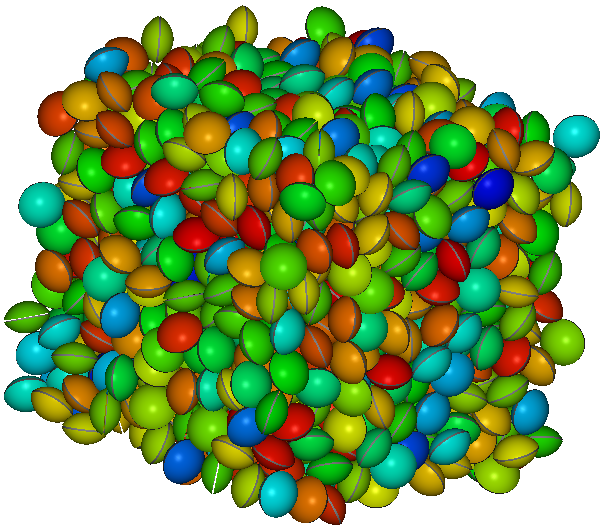
\includegraphics[width=\textwidth]{assets/images/cinacchi}
      \caption{Image by G. Cinacchi.}
      \label{fig:cinacchi_lens_provided}
    \end{subfigure}
    \begin{subfigure}{0.3\textwidth}
      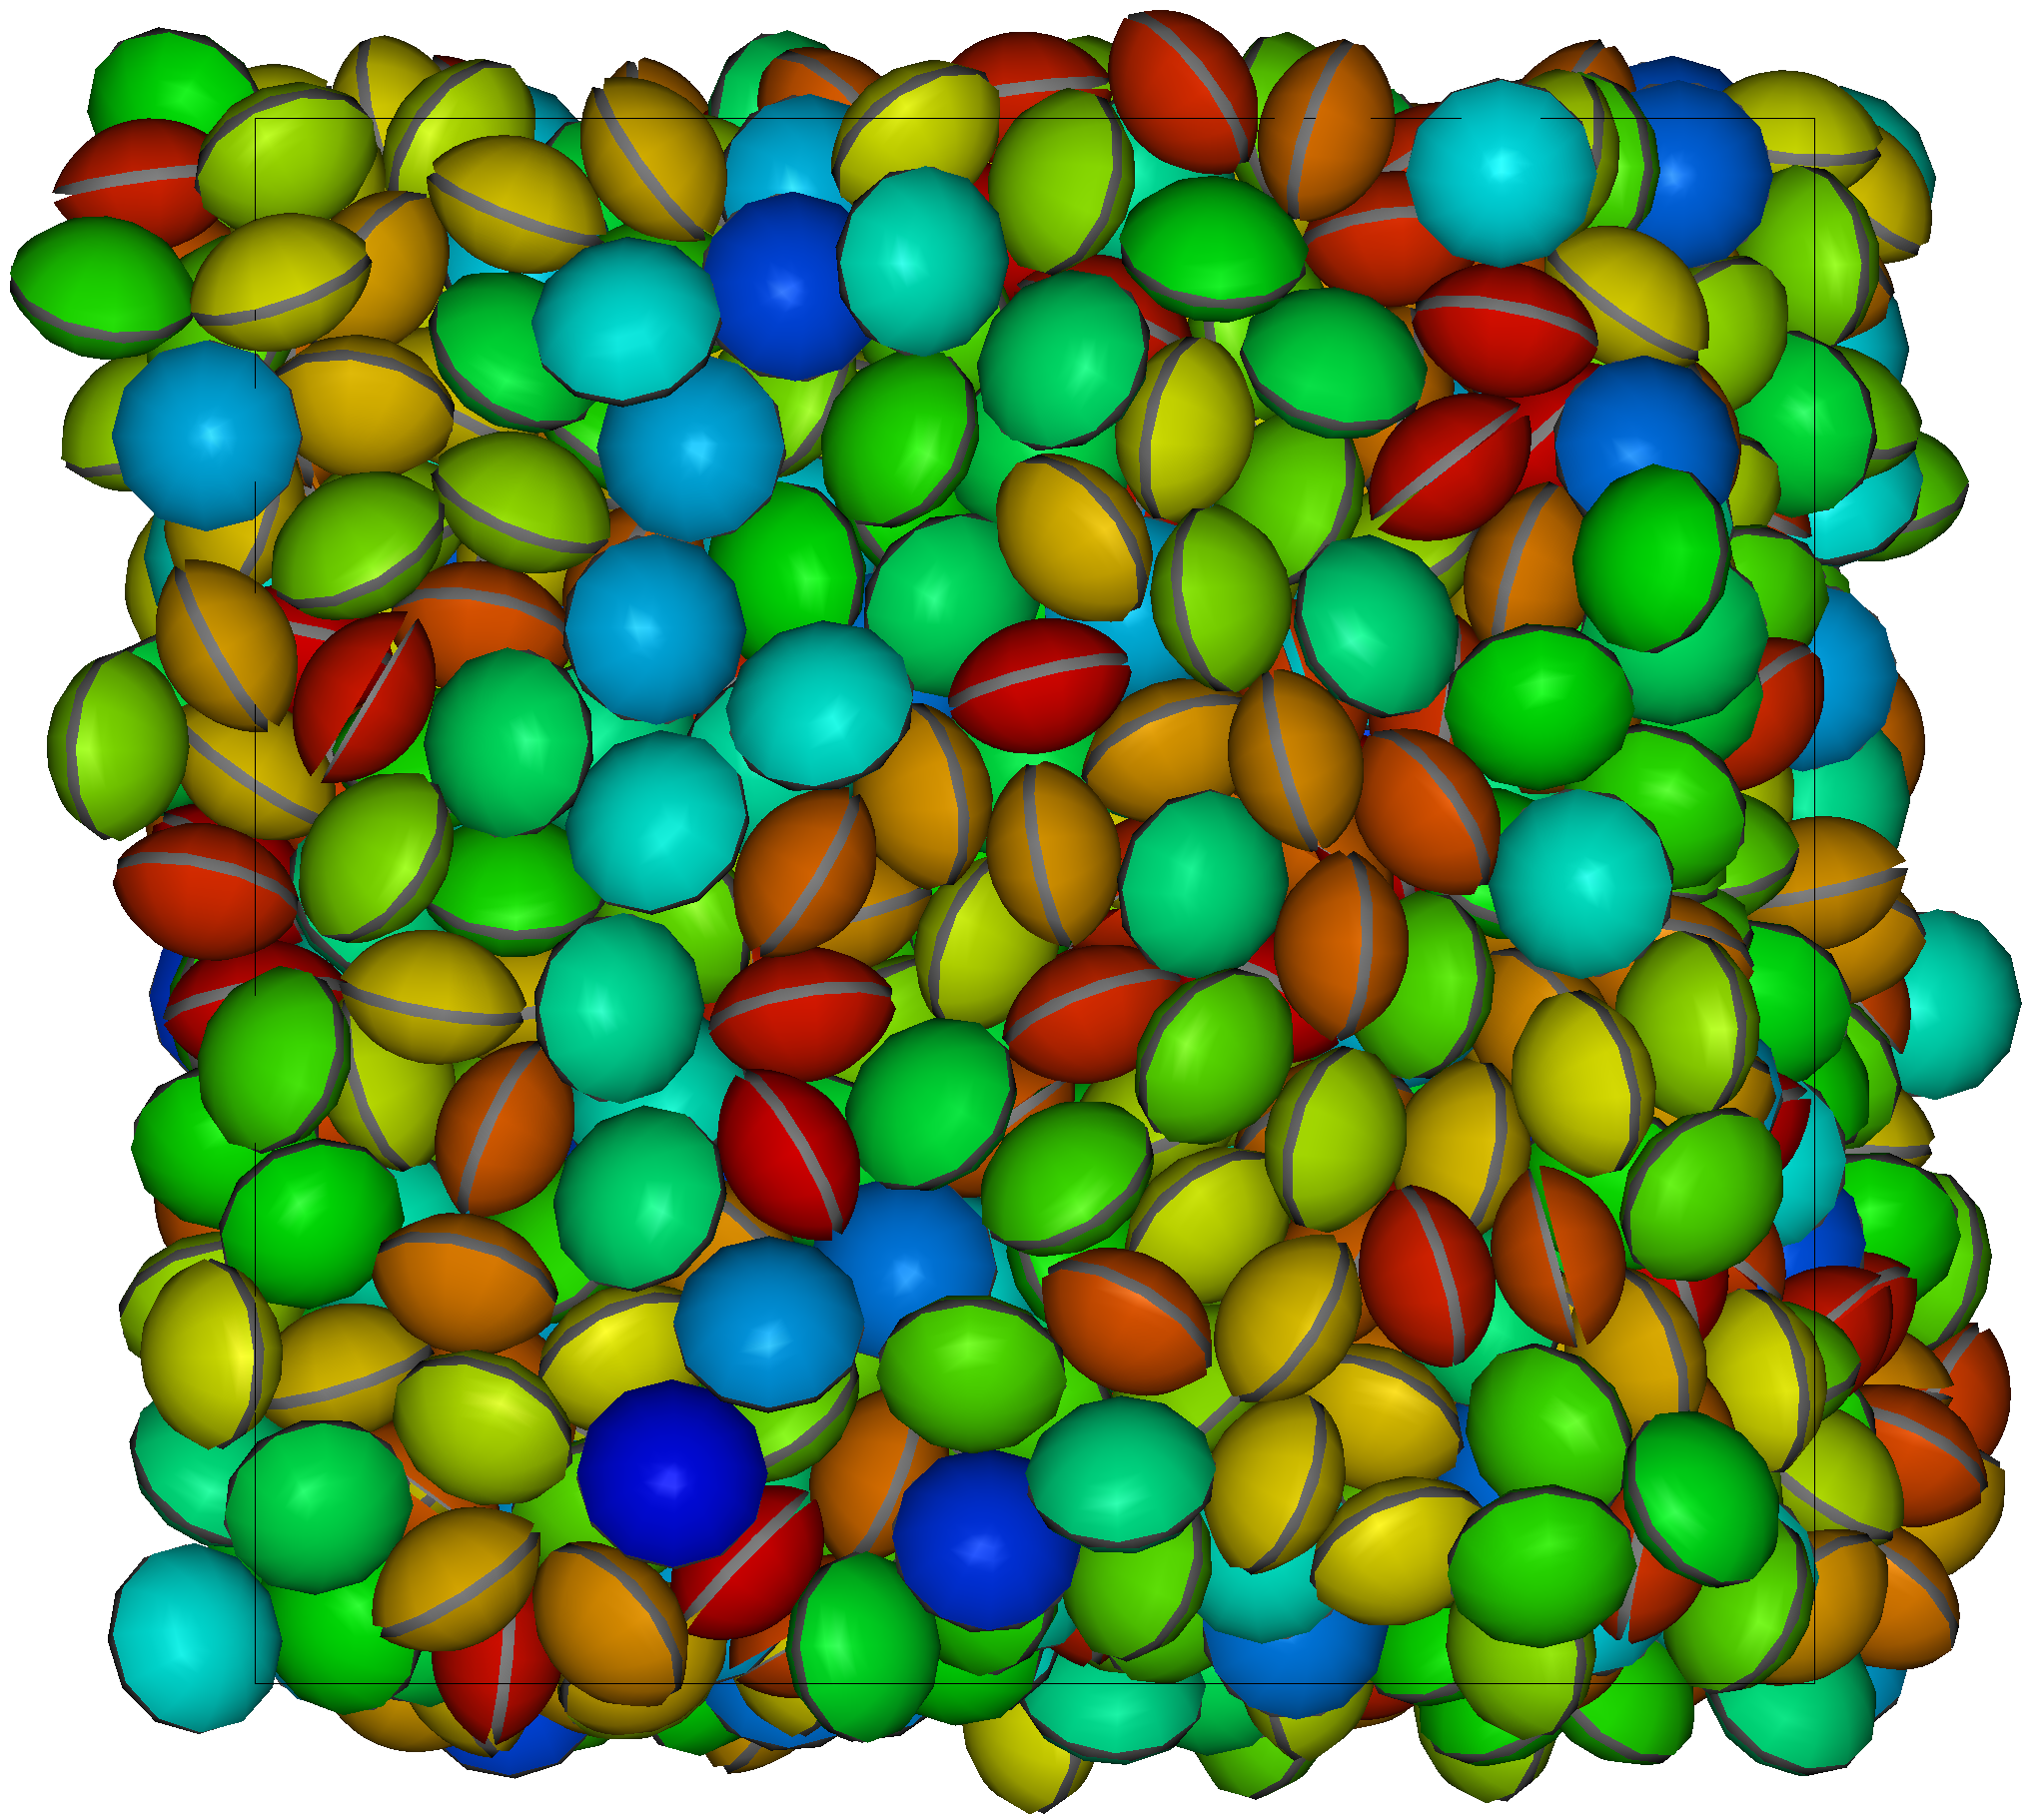
\includegraphics[width=\textwidth]{assets/images/qmga}
      \caption{QMGA recreation.}
      \label{fig:cinacchi_lens_qmga}
    \end{subfigure}
    \begin{subfigure}{0.3\textwidth}
      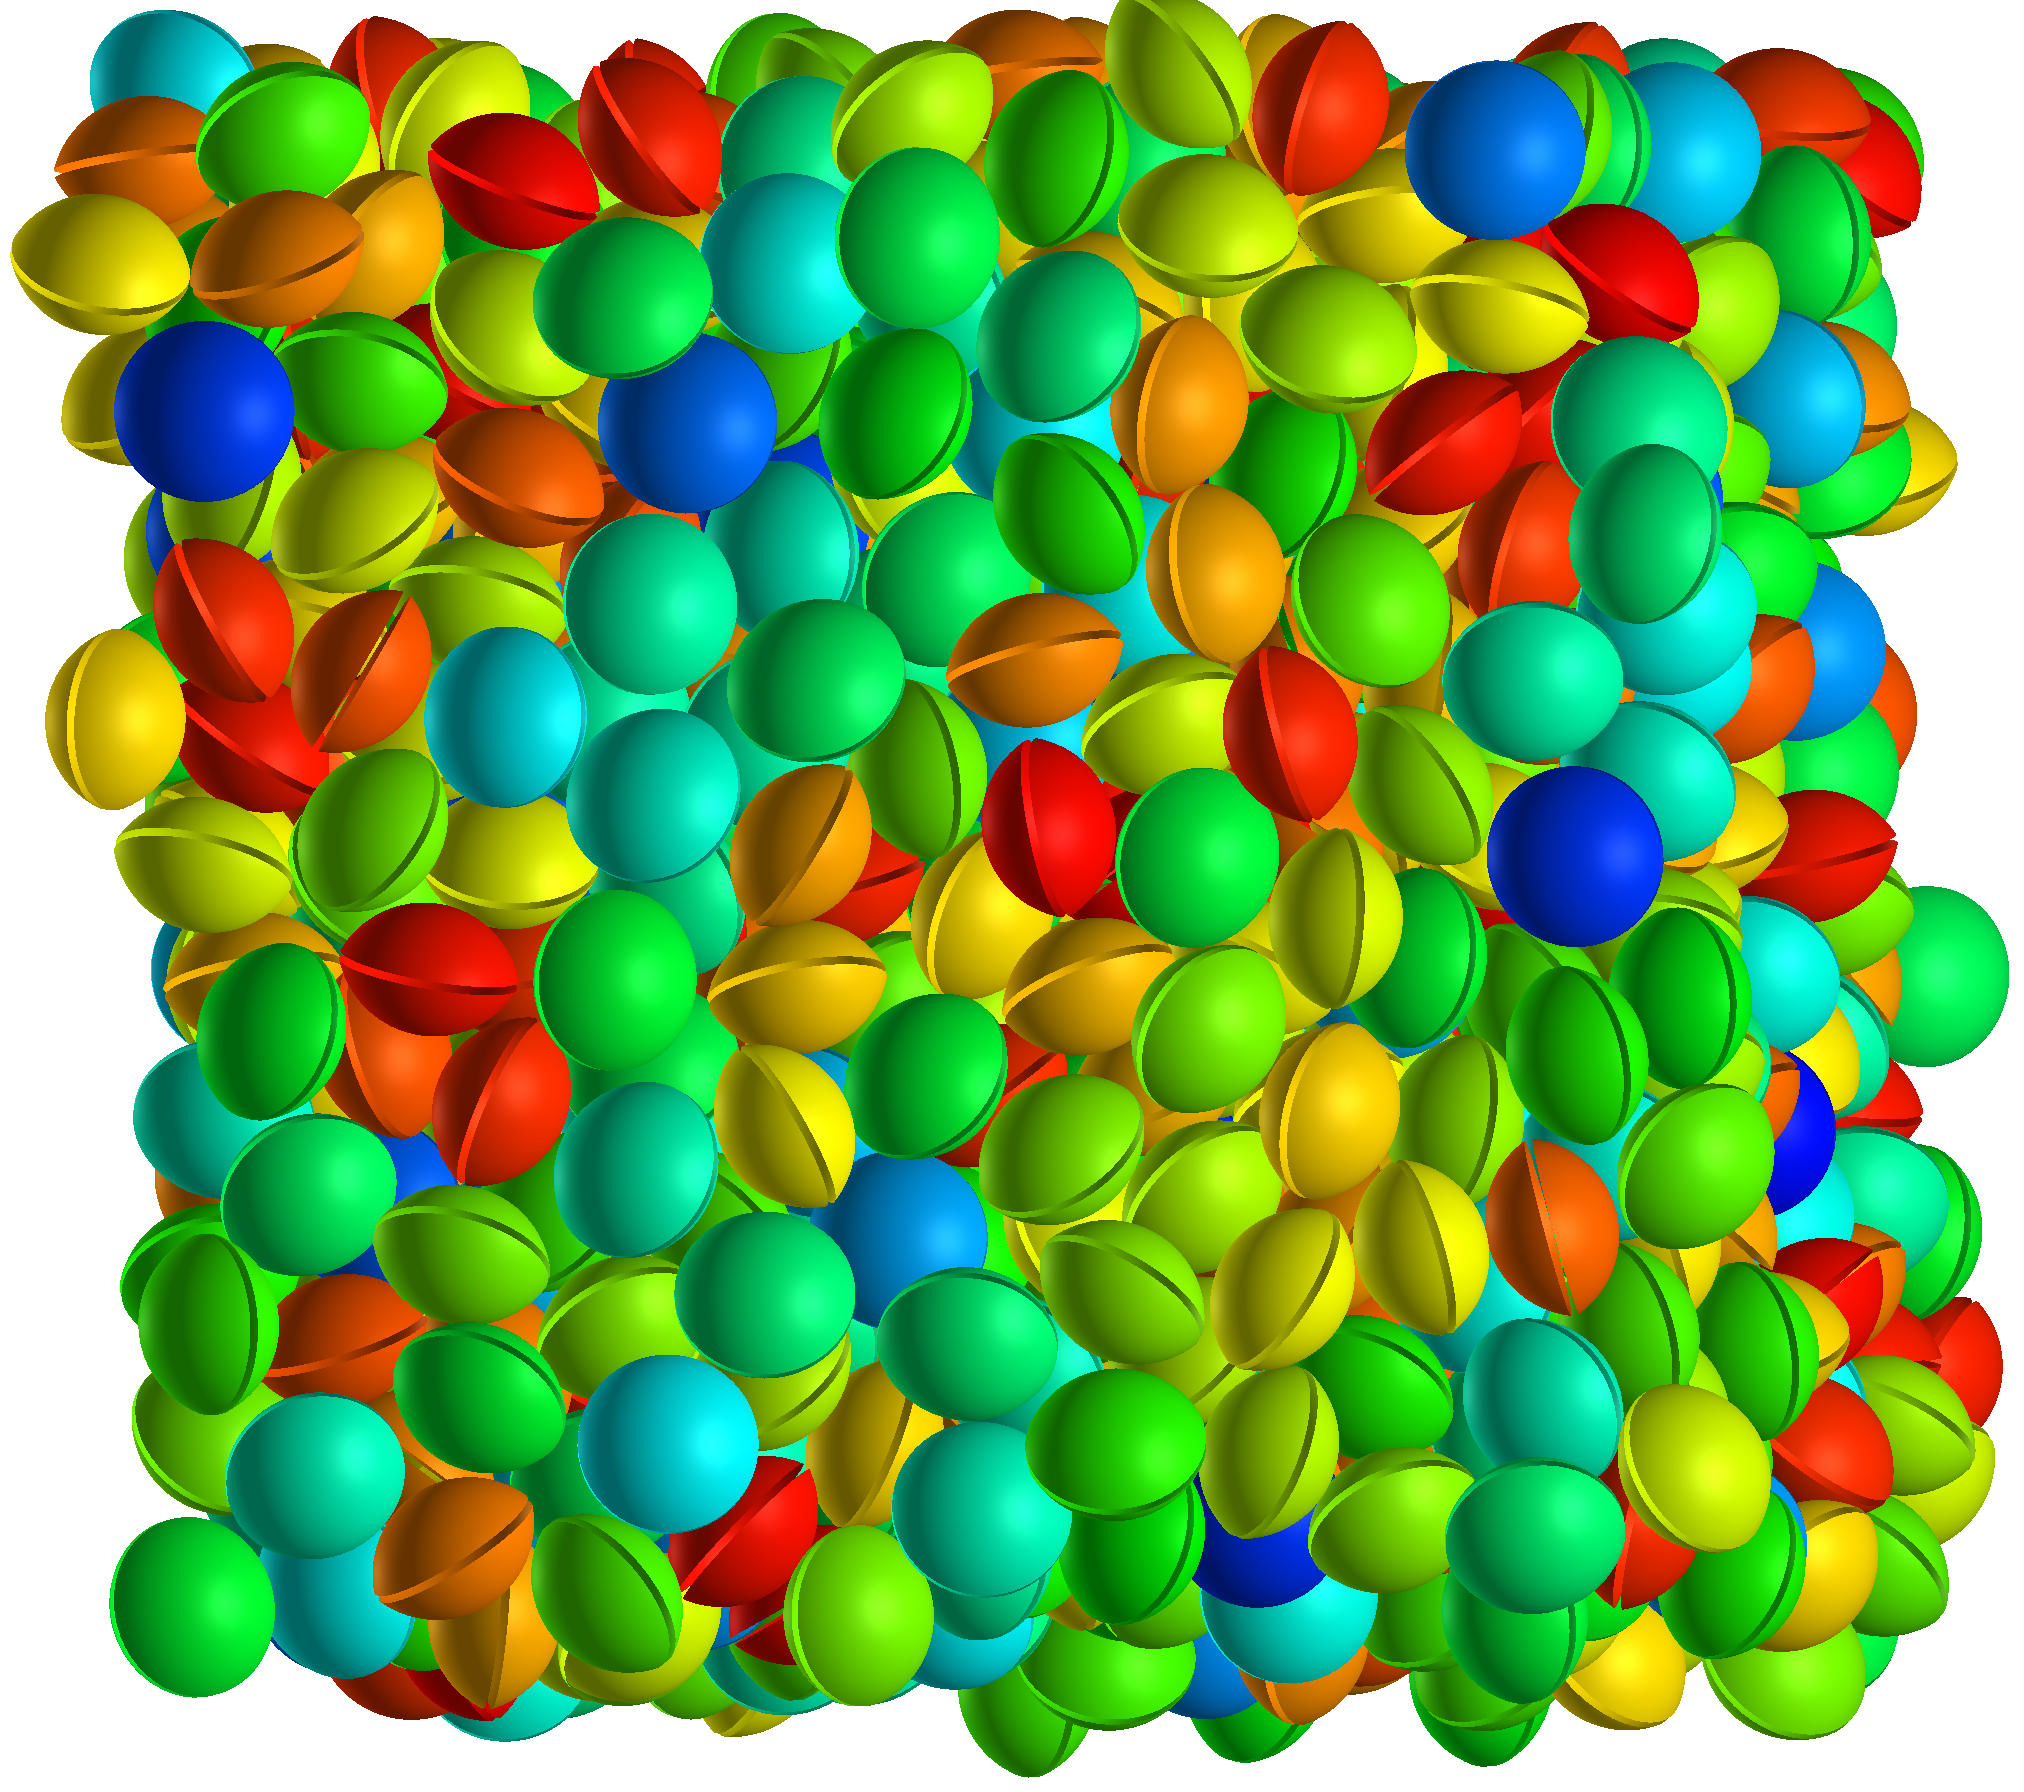
\includegraphics[width=\textwidth]{assets/images/webmga}
      \caption{WebMGA recreation.}
      \label{fig:cinacchi_lens_webmga}
    \end{subfigure}
  \end{center}
  \caption{Lens setup required by Giorgio Cinacchi.}
  \label{fig:cinacchi_lens}
\end{figure}

\subsubsection{Biconvex Lens}
\label{biconvex_section}
The biconvex lens shape (\cref{fig:biconvex_shape}, parameters ``Radius'', ``Angle'', ``Separation'') is implemented as a specific inititalisation of the ``BaseLens'' where $r_2=-r_1$.

Since the configurations provided by Cinacchi (\cref{fig:cinacchi_lens_provided}) aimed to emulate a biconvex lens using two separate lenses, but exhibited a small gap between the two parts, it was decided that a separation parameter would also be provided. This is implemented by moving the top part up and bottom part down by half the separation value. A row of vertices is inserted between to split the flat edge into triangles as seen in \cref{fig:new_biconvex_w}. A complication encountered is that by default the bottom half of the lens is not aligned correctly which results in a twisting effect visible in \cref{fig:bad_biconvex}, so all vertex rows must be shifted such that the correct configuration applies for triangle generation.
\newshapefigure{biconvex}{biconvex lens}
\begin{figure}
\begin{center}
    \begin{subfigure}{0.4\textwidth}
      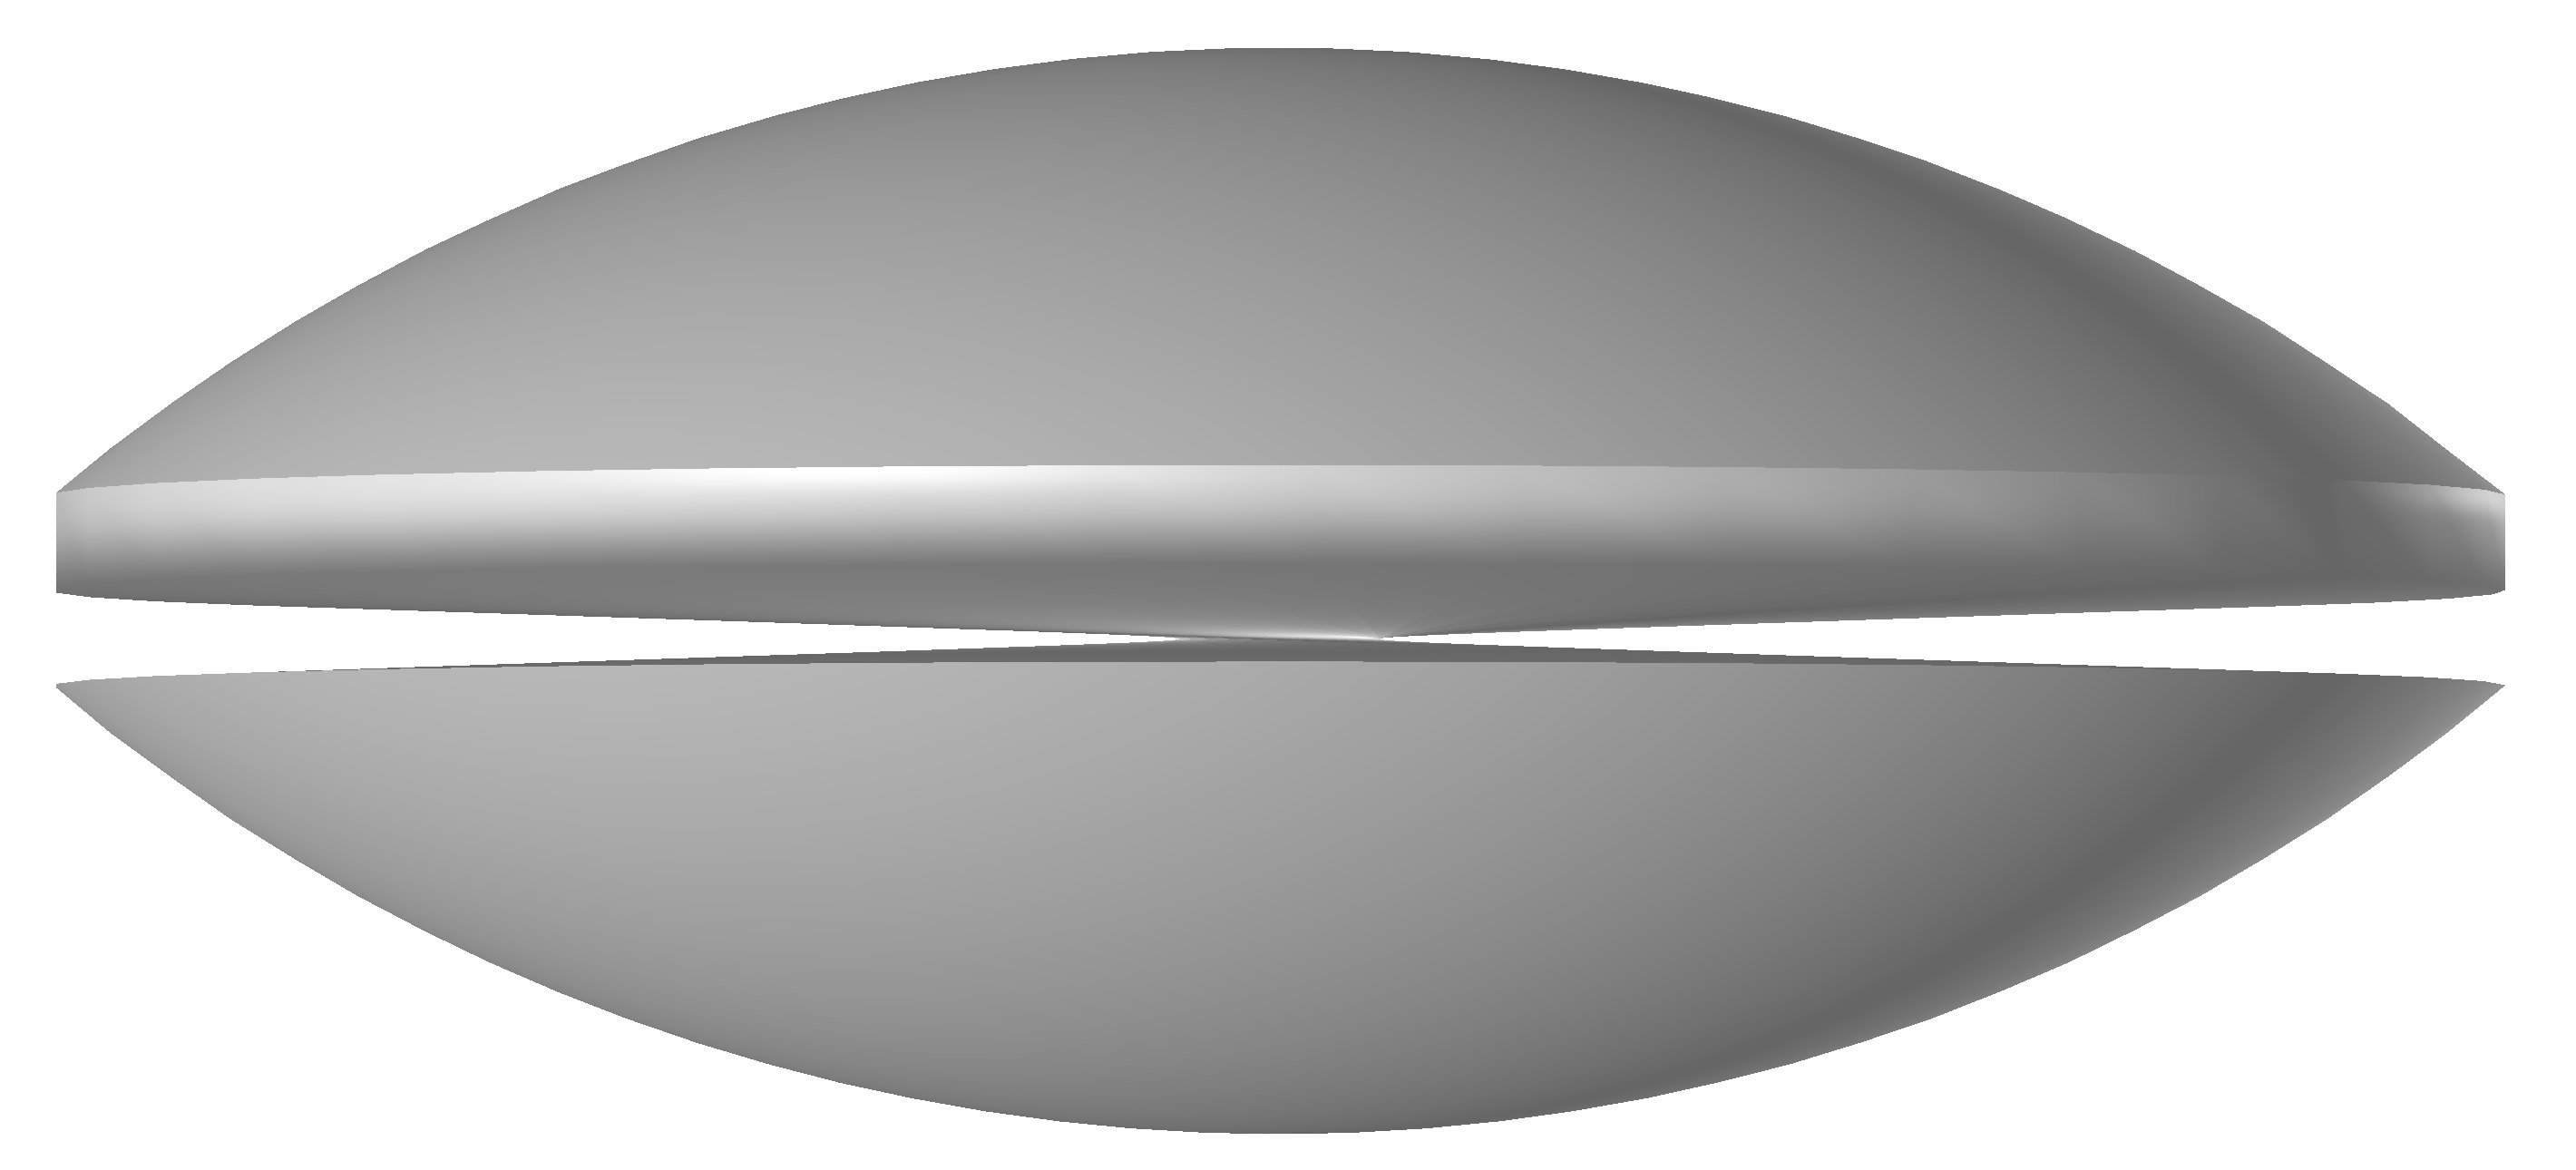
\includegraphics[width=\textwidth]{assets/images/shapes/bugnew/bicon}
      \caption{Shape.}
    \end{subfigure}
        \begin{subfigure}{0.4\textwidth}
      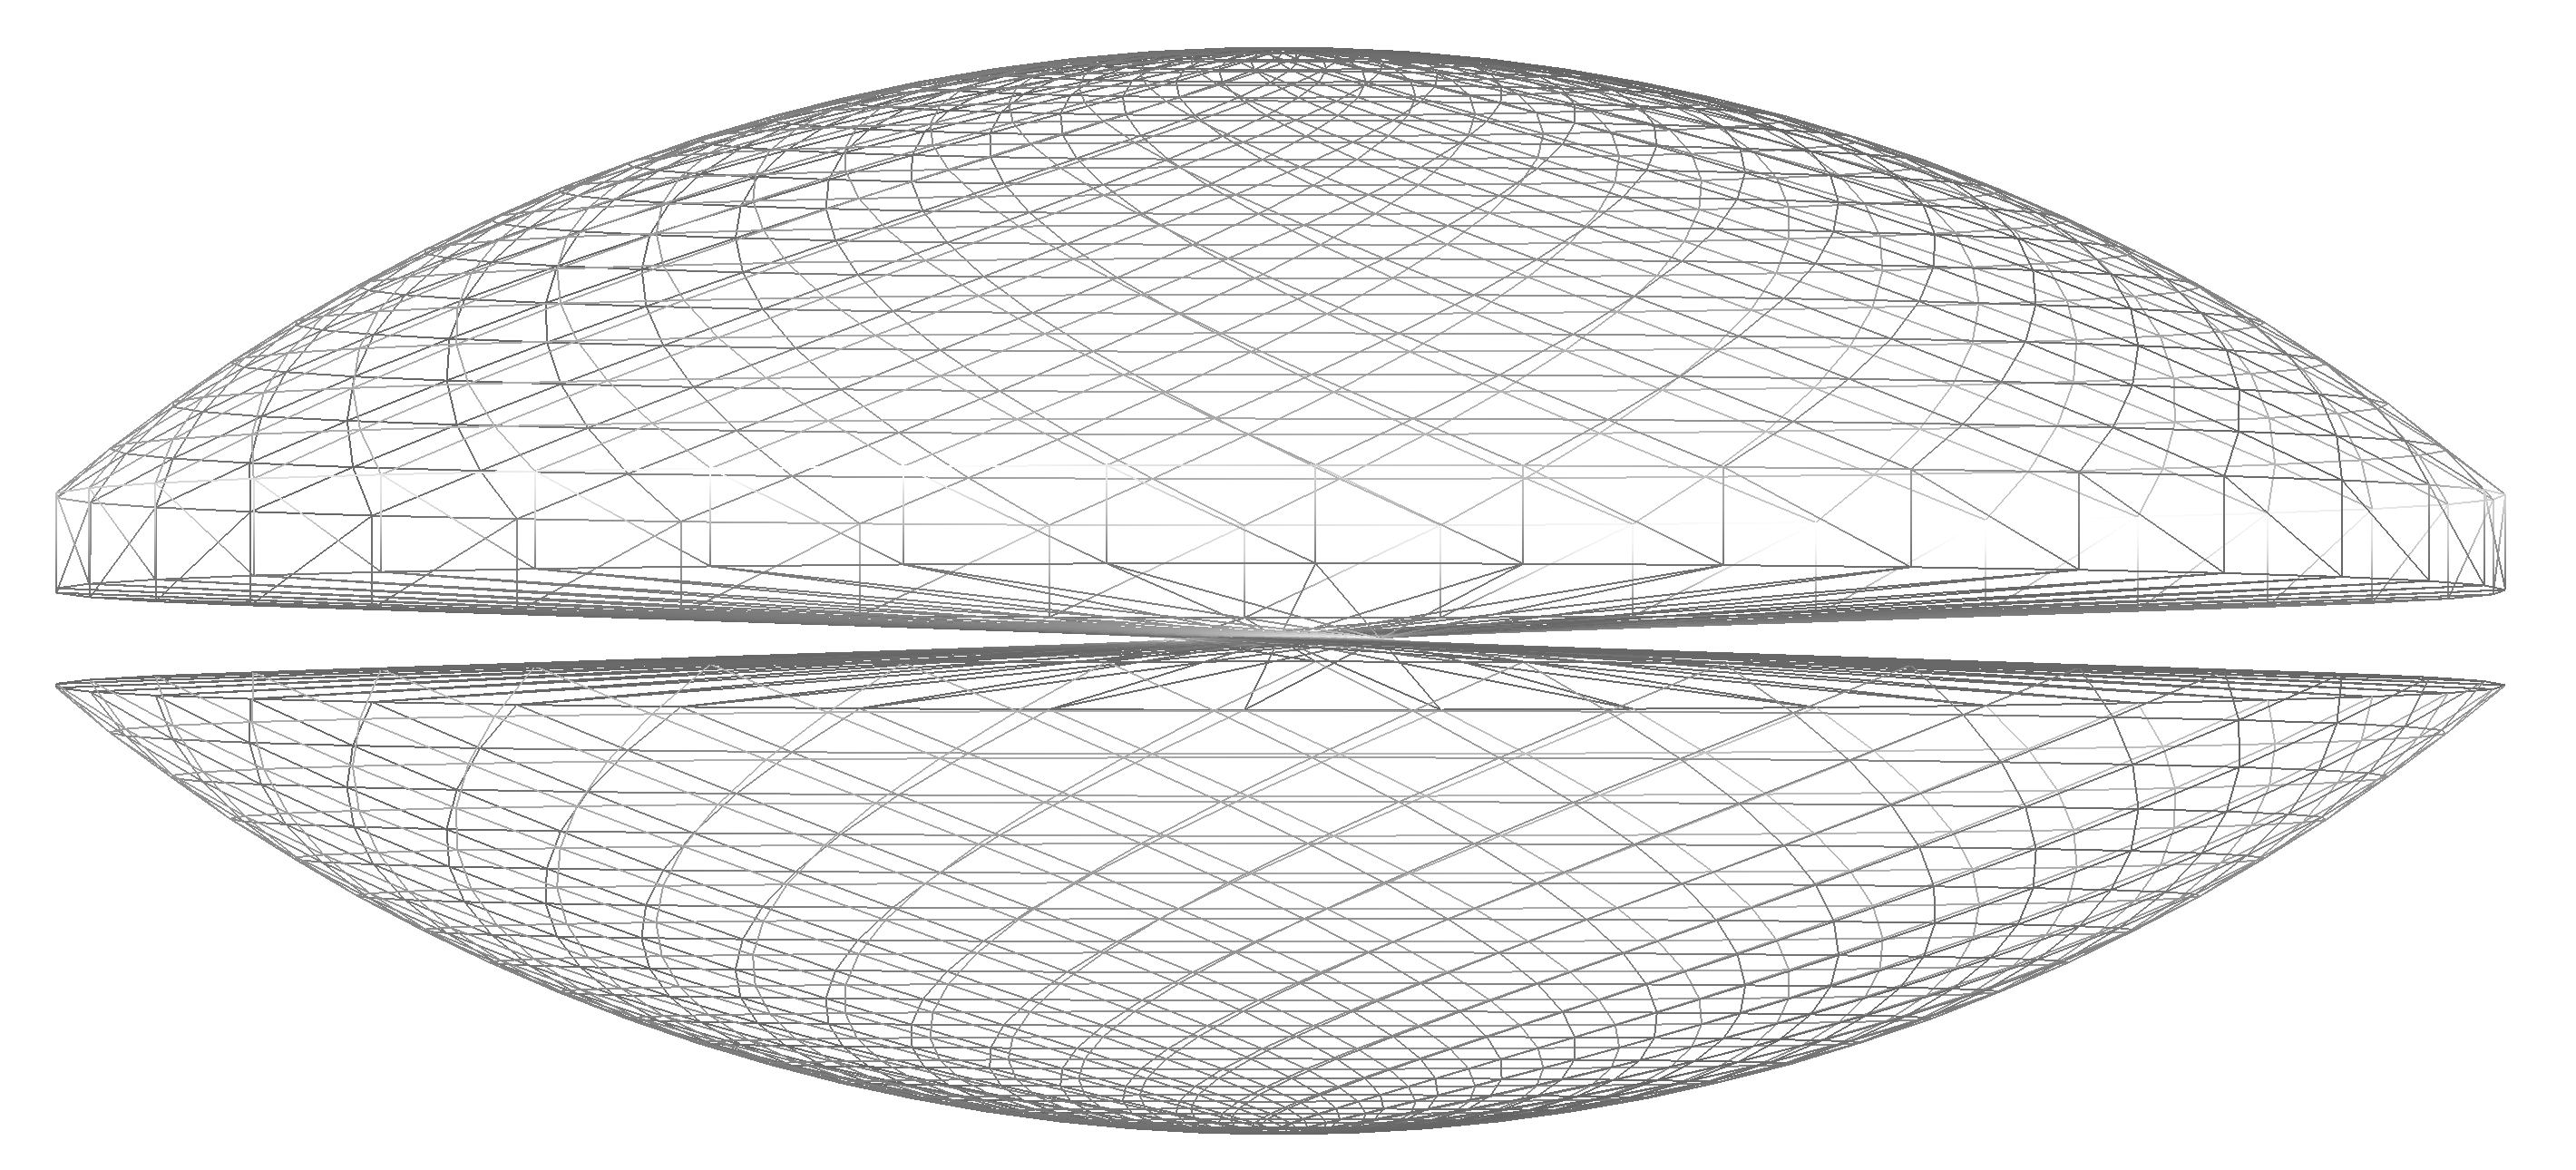
\includegraphics[width=\textwidth]{assets/images/shapes/bugnew/bicon_w}
      \caption{Wireframe.}
    \end{subfigure}
    \end{center}
  \caption{Incorrectly configured biconvex lens where halves are incorrectly aligned.}
  \label{fig:bad_biconvex}
\end{figure}

\subsubsection{Spherocylinder}
\label{spherocylinder_section}
The spherocylinder shape (\cref{fig:spherocylinder_shape}, parameters ``Radius'', ``Length'') can be represented as an origin centred sphere of radius $r$ scaled in the $z$ directions by (half of) some length value in each $z$ direction (positive/negative). This can be represented by a slightly modified form of the Cartesian sphere equation in \cref{sphere_equation_cartesian} (where $l$ denotes stretch length),

\begin{equation}
\mathbf{r}_\mathrm{c}=\begin{pmatrix}r\sin\phi \cos\theta\\
r\sin\phi \sin\theta\\
r\cos\theta + n\end{pmatrix}
=\mathbf{r}_\mathrm{C}+\begin{pmatrix}0\\
0\\
n\end{pmatrix}
\label{spherocylinder_equation}
\end{equation}
\begin{equation}
n=\begin{cases}
  \frac{l}{2}&\text{if } r\cos\theta>0\\
  -\frac{l}{2}&\text{if } r\cos\theta<0\\
  0&\text{otherwise.}
\end{cases}
\label{spherocylinder_n_equation}
\end{equation}.
\paragraph{Initial Attempt}

From \cref{spherocylinder_equation,spherocylinder_n_equation}, it can be seen that a spherocylinder can be approximated by slightly modifying the vertex sampling process for a sphere, whilst leaving the rest of the mesh building process unchanged. A sphere point can be sampled using \cref{sphere_equation_cartesian} with radius $r$ and added to the scaling vector $\begin{pmatrix}0,0,n\end{pmatrix}^\mathsf{T}$ as defined in \cref{spherocylinder_n_equation} to give an equivalent result to \cref{spherocylinder_equation}.

In the program this was implemented by creating a ``Spherocylinder'' class as a child of the ``Sphere'' class and overriding the ``sample\_sphere()'' method. Since this implementation is so simple, the JavaScript code is provided below:

\begin{adjustbox}{width=\textwidth}
\begin{lstlisting}
//Spherocylinder mesh generator
export class Spherocylinder extends Sphere {
    //Scaling vector (either side of centre) to stretch sphere into spherocylinder ([0, 0, length / 2])
    length_scaling_vector: number[];

    constructor(radius: number, length: number) {
        //Derive from origin centred sphere of chosen radius
        super(radius);
        this.length_scaling_vector = [0, 0, length / 2];
    }

    //Samples from spherocylinder instead of sphere
    sample_sphere(radius: number, theta: number, phi: number, epsilon: number = 1e-15): number[] {
        let sphere_coordinate: number[] = super.sample_sphere(radius, theta, phi);
        //Stretch point in z direction by scale vector, matching stretch direction to sign of original vertex z
        //Unchanged if z is (approximately) 0
        if (Math.abs(sphere_coordinate[2]) < epsilon) {
        } else if (sphere_coordinate[2] > 0) {
            sphere_coordinate = math.add(sphere_coordinate, this.length_scaling_vector);
        } else if (sphere_coordinate[2] < 0) {
            sphere_coordinate = math.subtract(sphere_coordinate, this.length_scaling_vector);
        }
        return sphere_coordinate;
    }
}
\end{lstlisting}
\end{adjustbox}

\begin{figure}
  \begin{center}
    \begin{subfigure}{0.3\textwidth}
      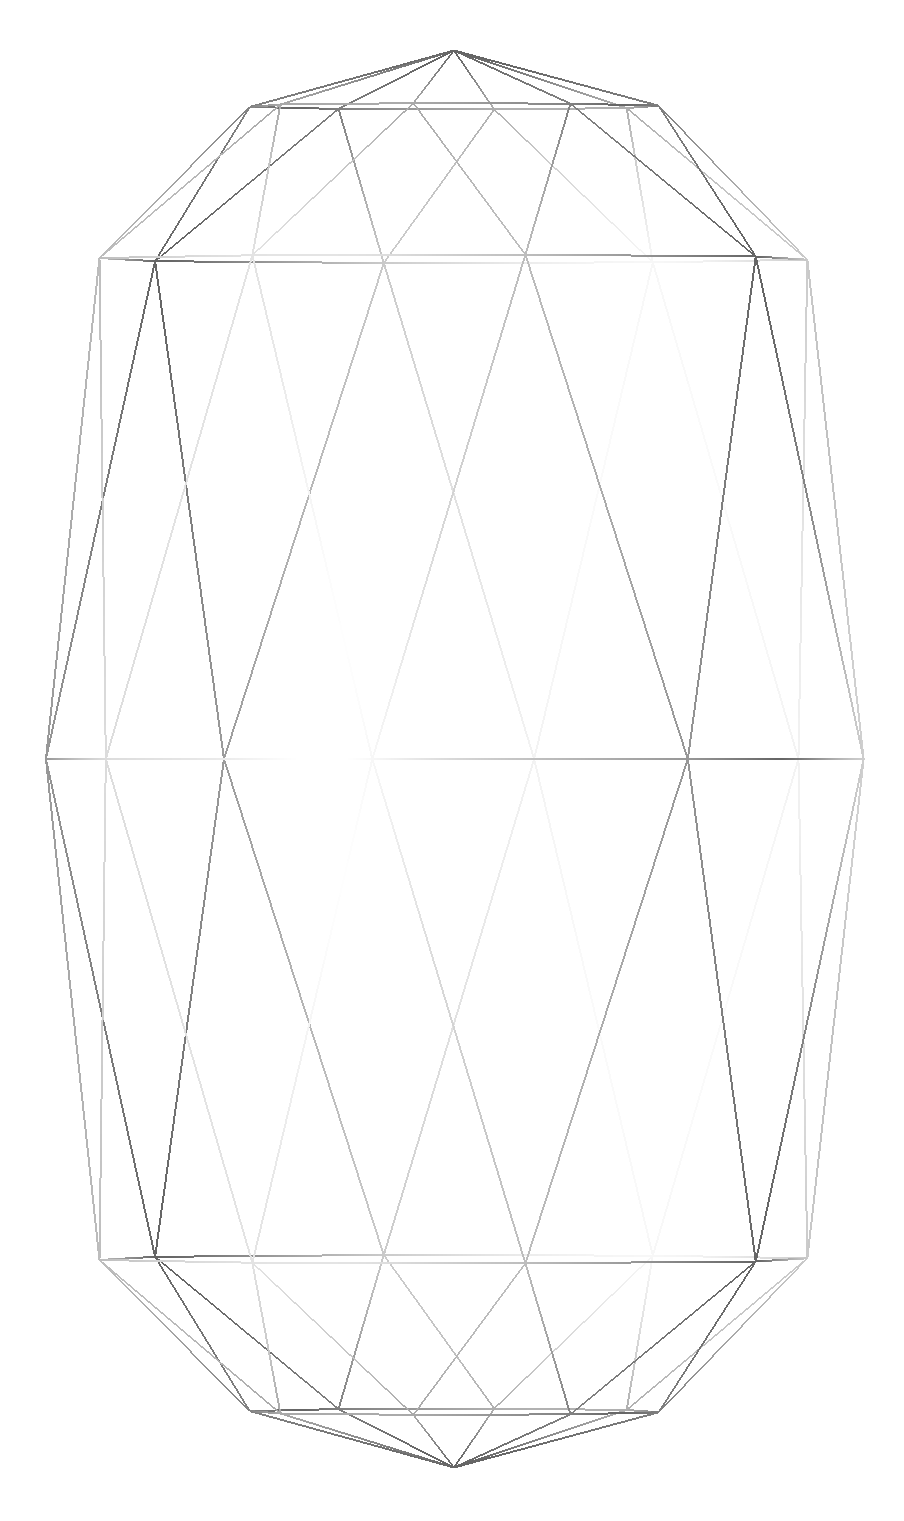
\includegraphics[width=\textwidth]{assets/images/shapes/sphero_bug/low_2}
      \caption{\makefirstuc{Low mesh density.}}
      \label{fig:sphero_bug_low_2}
    \end{subfigure}
        \begin{subfigure}{0.3\textwidth}
      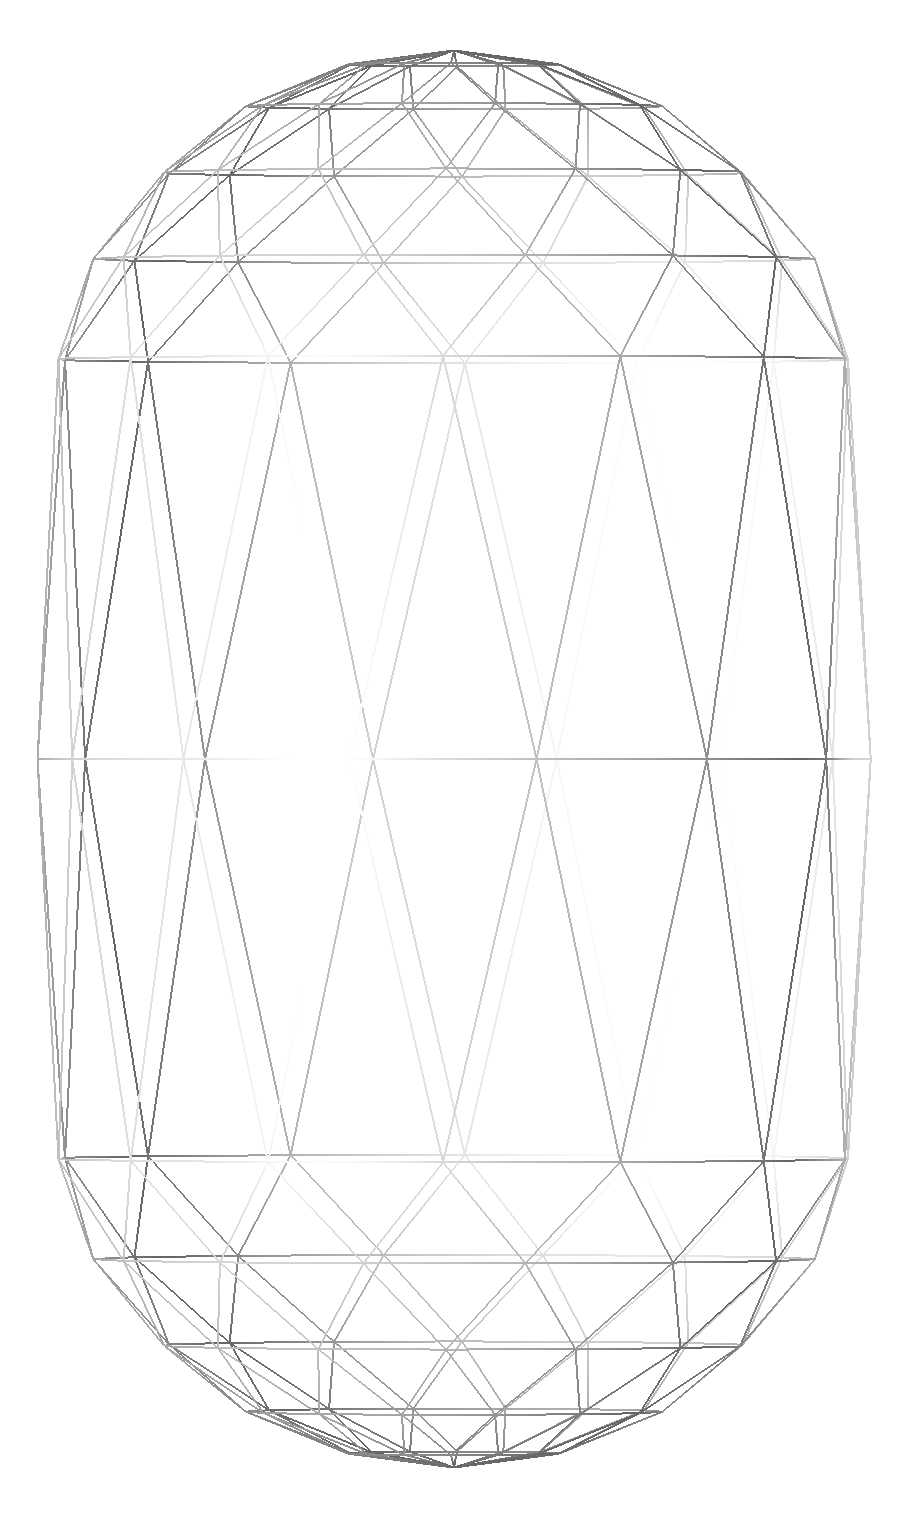
\includegraphics[width=\textwidth]{assets/images/shapes/sphero_bug/med_2}
      \caption{\makefirstuc{Medium mesh density.}}
      \label{fig:sphero_bug_med_2}
    \end{subfigure}
        \begin{subfigure}{0.3\textwidth}
      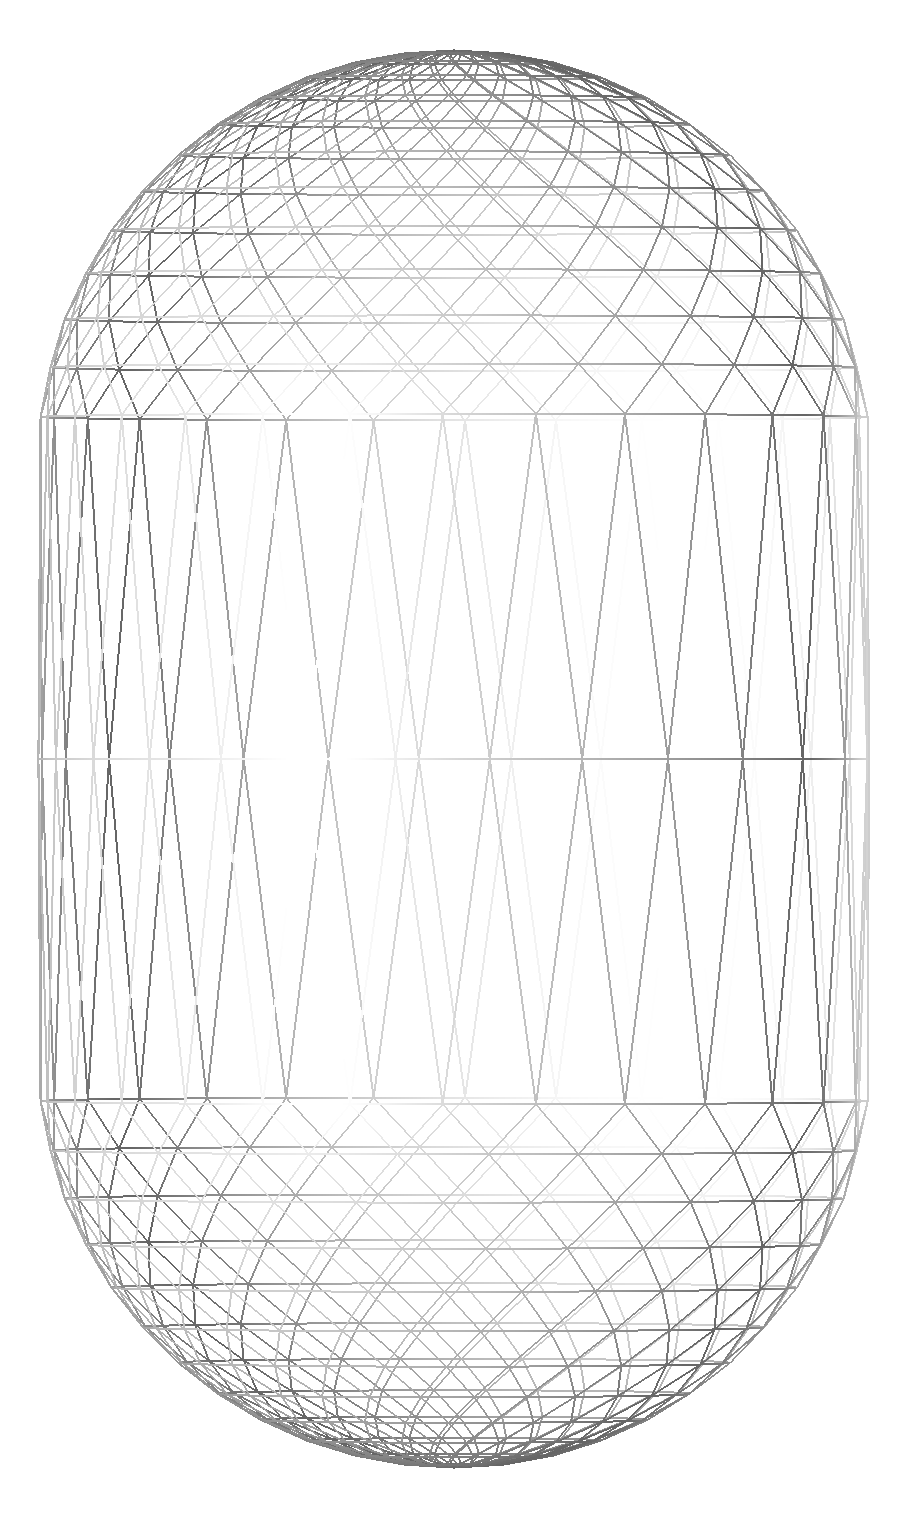
\includegraphics[width=\textwidth]{assets/images/shapes/sphero_bug/high_2}
      \caption{\makefirstuc{High mesh density.}}
      \label{fig:sphero_bug_high_2}
    \end{subfigure}
  \end{center}
  \caption{Initial spherocylinder implementation. Visible tapering can be observed, particularly with low mesh density.}
  \label{fig:sphero_bug}
\end{figure}
Unfortunately, this process produced visually unsatisfying results with the sides of the spherocylinder visibly tapering, particularly with low detail meshes. This can be seen in \cref{fig:sphero_bug}. After producing the biconvex lens, an alternate, much simpler solution became apparent which avoided this issue.
\paragraph{Second Attempt}

A spherocylinder can also be considered a special case of the biconvex lens. A biconvex lens with no separation and aperture angle $\frac{\pi}{2}$ produces a sphere with the given radius $r$. Increasing the separation parameter causes the two hemispheres to move apart such that a spherocylinder is produced. The spherocylinder can therefore simply be considered a special case of the biconvex lens with aperture angle $\frac{\pi}{2}$, and can be implemented entirely through class inheritance as shown:
\begin{lstlisting}
//Spherocylinder mesh generator
export class Spherocylinder extends BiconvexLens {
    constructor(radius: number, length: number) {
        super(radius, Math.PI / 2, length);
    }
}
\end{lstlisting}
This produced the result shown in \cref{fig:spherocylinder_shape}.
\shapefigure{spherocylinder}{spherocylinder}

\subsection{WebMGA 3.0 Bugs}
\label{shape_bug_spher}
Most shapes were successfully implemented fully and appear as expected. The shading on the spherocylinder in \cref{fig:new_spherocylinder} appears slightly incorrect at the boundary between the curved section and the flatter section, however this is more subtle than WebMGA 2.0's incorrect spherocylinder mesh. A fix for this should be investigated. It likely arises due to some error in calculation of vertex normals.
